\documentclass[10pt,journal,letterpaper]{IEEEtran}

\usepackage[english]{babel}
\usepackage{svg}
\usepackage{cite}
\usepackage{amsmath}
\usepackage{graphicx}
\usepackage[hidelinks]{hyperref}
\usepackage{booktabs}    % 优美表格线
\usepackage{multirow}    % 合并行
\usepackage{amssymb}     % √ 符号
\usepackage{makecell}  
\usepackage{array}       % 控制列宽
\usepackage{xcolor}
\usepackage[caption=false, font=footnotesize]{subfig}
\usepackage[linesnumbered,ruled,vlined]{algorithm2e}
\usepackage[most]{tcolorbox}
\usepackage{tabularx}

\newtcolorbox{observationbox}[1]{
    colback=gray!4,
    colframe=black!55,
    boxrule=0.6pt,
    arc=1.5pt,
    left=5pt,
    right=5pt,
    top=4pt,
    bottom=4pt,
    title=\textbf{#1},
    fonttitle=\normalsize,
    coltitle=black,
    colbacktitle=gray!18
}

\newenvironment{observation}[1][Observation]
{\begin{observationbox}{#1}}
{\end{observationbox}}




\title{vLLM-FI: A Fault Injection Framework for Reliability Evaluation of LLM Inference}
\author{Jie~Ren,
Zizhen~Liu,~\IEEEmembership{Member,~IEEE,}
Songwei~Pei,~\IEEEmembership{Member,~IEEE,}
Cheng~Liu,~\IEEEmembership{Senior~Member,~IEEE,}
Huawei~Li,~\IEEEmembership{Senior~Member,~IEEE,}
and Shangguang~Wang,~\IEEEmembership{Senior~Member,~IEEE}%
\thanks{Jie Ren, Songwei Pei, and Shangguang Wang are with Beijing University of Posts and Telecommunications, Beijing, China.}%
\thanks{Zizhen Liu and Huawei Li are with the Institute of Computing Technology, Chinese Academy of Sciences, Beijing, China.}%
\thanks{Cheng Liu is with North China Electric Power University, China.}%
\thanks{Corresponding authors: Songwei Pei and Cheng Liu.}}


\begin{document}
\markboth{IEEE Transactions on Computer-Aided Design of Integrated Circuits and Systems}%
{Ren \MakeLowercase{\textit{et al.}}: vLLM-FI for Reliability Evaluation of LLM Inference}
\maketitle

\begin{abstract}
Transient hardware faults threaten large language model (LLM) inference, where autoregressive decoding and multi-GPU execution allow errors to propagate across tokens and devices. Existing model-level fault-injection tools provide limited support for distributed and quantized inference, often overlook computation-dependent fault exposure and communication faults, and incur repeated host--device transfers for bit mutation. We present vLLM-FI, a fault-injection and reliability-evaluation framework integrated with vLLM. The framework models memory, computation, and communication faults, accounting for computational exposure beyond output tensor size and perturbing software-visible communication buffers. Configuration-driven targeting coordinates injection across distributed workers, while customized CUDA operators flip bits in place on GPU-resident tensors. Support for tensor and pipeline parallelism, quantized representations, and standardized downstream-task evaluation enables systematic reliability studies under practical inference configurations. In calibration experiments, vLLM-FI matches MRFI's output-level fault effects with a maximum absolute difference of 0.62 percentage points in fault-injection correct rate. Across the evaluated all-layer projection-injection workloads, vLLM-FI achieves a $1.81\times$--$2.41\times$ end-to-end speedup over MRFI. With the inference runtime held fixed, GPU-resident injection delivers up to a $5.22\times$ speedup in total experiment runtime over an MRFI-style CPU-mediated backend under compute-fault injection. These results demonstrate lower experimental cost while preserving agreement with the reference injector under the tested settings, enabling broader reliability evaluation across fault models, tasks, quantization methods, and parallel configurations.
\end{abstract}

\begin{IEEEkeywords}
Fault injection, reliability evaluation, large language models, distributed inference, GPU computing, quantization.
\end{IEEEkeywords}





\section{Introduction}

Transient hardware faults remain an important threat to computing-system reliability. Continued device scaling, higher integration density, and lower operating voltages may increase hardware susceptibility to soft errors \cite{mukherjee2005soft,borkar2006designing,baumann2005radiation,frustaci2015sram}, while physical drift in emerging memory devices may also induce data bit flips \cite{yilmaz2017drift,junsangsri2014new}. These faults may manifest as silent data corruption (SDC), producing incorrect results without triggering observable failures. This concern is particularly important for large language models (LLMs). Built primarily on the Transformer architecture \cite{vaswani2017attention}, LLMs have demonstrated strong capabilities across language understanding, generation, and reasoning tasks \cite{brown2020language,zhao2023survey}. During autoregressive inference, model layers are executed repeatedly, allowing perturbations in parameters, activations, or intermediate results to propagate across decoding steps. Moreover, increasing model sizes are driving LLM inference toward multi-GPU deployment, where faults may also occur and propagate across devices.

Existing neural-network reliability studies have developed various fault injection tools for convolutional neural networks (CNNs) and conventional deep neural networks (DNNs) \cite{mahmoud2021optimizing,wan2024mulberry,jiao2017assessment,liu2022special,xu2021reliability,reagen2018ares,mahmoud2020pytorchfi,huang2024mrfi}. However, these tools provide limited native support for important characteristics of modern LLM inference, including distributed parallelism, quantized model representations, and iterative decoding. In contrast, vLLM incorporates parallelism, quantization, and system optimizations within a common inference architecture \cite{kwon2023efficient}, making it a suitable foundation for fault injection under practical LLM inference configurations.

Two additional limitations prevent traditional approaches from scaling effectively to distributed LLM inference. First, existing model-level fault models commonly determine the number of computation faults from the number of elements in an operation's output tensor. Output size, however, does not reflect the underlying computational exposure: operations with the same output dimensions may require substantially different numbers of multiply--accumulate operations. Furthermore, communication-buffer faults are rarely covered, leaving an important fault source in multi-GPU inference insufficiently represented. Second, a common injection path transfers selected GPU tensor values to the CPU for bit-level modification and then copies them back to the GPU. This implementation is simple and can be acceptable for relatively small CNN and DNN workloads with limited forward execution and sparse fault injection. For LLMs, however, large tensors, iterative decoding, and increasing fault counts repeatedly introduce host--device transfers and synchronization, causing the injection overhead to grow rapidly. Direct GPU modification avoids this path but requires careful handling of data-type representations, concurrent updates, and asynchronous CUDA execution.

To address these challenges, we present vLLM-FI, a fault-exposure-aware runtime fault injection and reliability evaluation framework integrated with vLLM. vLLM-FI extends model-level fault injection to cover memory, computation, and communication faults. Its computation fault model accounts for computational exposure beyond output tensor size, while its communication fault model supports injection into software-visible communication buffers. To reduce injection overhead, vLLM-FI uses customized CUDA operators to perform in-place bit flips on GPU-resident tensors. Because vLLM executes models through distributed GPU workers, vLLM-FI employs a configuration-driven architecture to coordinate fault settings across processes and resolve them to the intended injection locations. The framework supports tensor parallelism, pipeline parallelism, and multiple full-precision and quantized model representations. It also integrates with lm-evaluation-harness, connecting configurable fault injection experiments with standardized downstream-task evaluation.

The main contributions of this paper are summarized as follows:

\begin{itemize}
    \item We develop fault-exposure-aware models for distributed LLM inference, covering memory, computation, and communication faults. The models derive compute-fault counts from runtime multiply--accumulate workloads rather than output size alone, and communication-fault counts from buffer sizes in tensor-parallel collectives and pipeline-stage transfers.

    \item We design a vLLM-native fault injection architecture that supports distributed and quantized LLM inference. Customized CUDA operators perform efficient in-place bit flips on GPU-resident tensors, while configuration-driven targeting coordinates fault injection across distributed execution processes.

    \item We integrate vLLM-FI with lm-evaluation-harness to provide an end-to-end workflow from fault configuration and injection to standardized reliability evaluation. We validate the framework and analyze LLM reliability across fault models, downstream tasks, quantization strategies, and model-parallel configurations. vLLM-FI is released as open source to support reproducible research.
\end{itemize}

% Queue Figure 1 early for placement at the top of page 3.
% Queued after the introduction so this two-column float appears on page 3.
\begin{figure*}[!t]
    \centering
    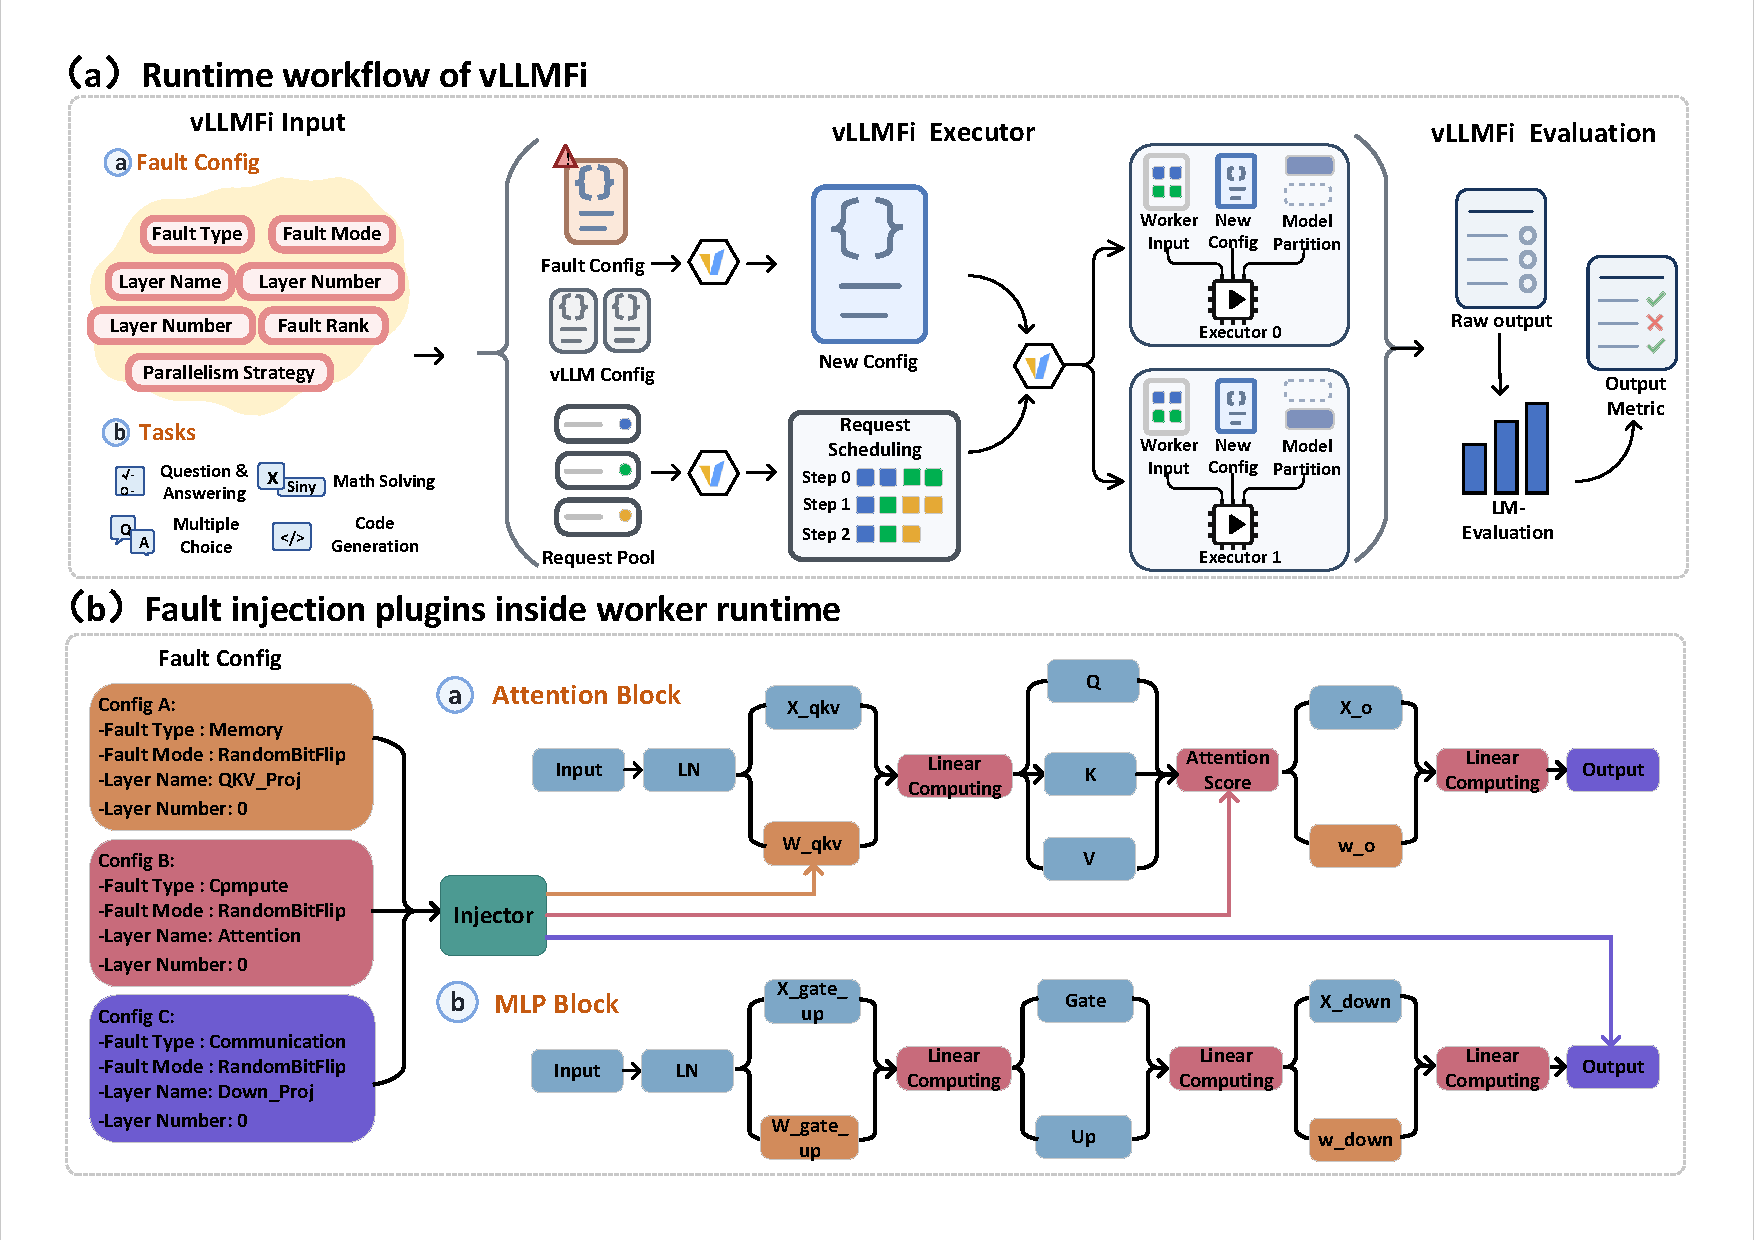
\includegraphics[
        width=\textwidth,
        trim=6pt 4pt 6pt 4pt,
        clip
    ]{vLLMFI.pdf}
    \caption{\textbf{Overview of vLLM-FI.}
    (a) Overall workflow: fault configuration and task inputs, distributed execution through the vLLM-FI executor, and task-level scoring through vLLM-FI evaluation.
    (b) Injection locations within Worker-side model computation, illustrated by QKV projection weights, an attention-computation result, and the MLP down-projection output buffer for memory, compute, and communication faults, respectively.}
    \label{fig:vllmfi_architecture}
\end{figure*}
\section{Related Work}

This section reviews two lines of research relevant to vLLM-FI: fault injection techniques and neural-network reliability analysis. The former concerns how hardware faults are represented and injected, whereas the latter examines how injected faults affect model behavior. We focus on their applicability to quantized and distributed LLM inference.

\subsection{Fault Injection Tools}

Fault injection techniques can be broadly categorized into hardware-level and model-level approaches. Hardware-level tools introduce faults into instructions, registers, or architectural states. GPU-Qin uses a GPU debugger, LLFI-GPU relies on compiler instrumentation, and SASSIFI injects faults at the SASS instruction level \cite{fang2014gpu,li2016understanding,hari2017sassifi}. NVBitFI builds on NVBit's dynamic binary instrumentation to provide configurable GPU fault injection \cite{villa2019nvbit,tsai2021nvbitfi}. These approaches retain detailed information about hardware-level fault behavior, but their cost increases with the number of dynamic instructions and kernel invocations. A recent study using NVBitFI found full-dataset LLM evaluation prohibitively time-consuming and therefore restricted its experiments to a limited set of inputs \cite{chai2026analysis}. This overhead makes hardware-level injection difficult to apply to large statistical campaigns involving autoregressive LLM inference.

Model-level approaches improve experimental efficiency by mapping hardware faults to perturbations of model parameters, activations, or intermediate tensors. Ares showed that model-level injection can reproduce statistical behaviors consistent with hardware faults \cite{reagen2018ares}, while PyTorchFI established a widely used runtime injection mechanism based on PyTorch hooks \cite{mahmoud2020pytorchfi}. More recent studies have extended model-level injection to language models. Sun et al. modified model weights and intermediate layer outputs to study LLM reliability \cite{sun2025demystifying,sun2025ft2}. ReaLM models the mixed-precision computation flow of SmoothQuant \cite{xiao2023smoothquant} and injects errors into INT32 accumulation results \cite{xie2025realm}. These studies demonstrate that model-level abstraction provides a practical basis for large-scale reliability analysis.

However, existing model-level tools remain only partially aligned with modern LLM inference systems. Most are built on standard PyTorch or Hugging Face Transformers execution paths and do not natively coordinate injection targets across distributed devices and execution stages. Supporting quantized inference generally requires separate implementations for individual quantization methods and their data representations. Moreover, existing rate-based fault models commonly determine the number of injected faults from tensor or output size, without reflecting the computation required to produce the output or the communication volume between devices. The representative tools in Table~\ref{tab:comparison} also lack communication-buffer fault injection and an in-place GPU injection path integrated with a distributed inference engine. Consequently, they do not jointly provide fault models that account for computation and communication volume, distributed target control, support for multiple quantization methods, and efficient GPU-resident injection.

Table~\ref{tab:comparison} compares vLLM-FI with representative model-level fault injection approaches.

\begin{table}[htbp]
\centering
\caption{Comparison of vLLM-FI with representative model-level fault injection approaches.}
\label{tab:comparison}
\renewcommand{\arraystretch}{1.25}
\setlength{\tabcolsep}{3pt}

\resizebox{\linewidth}{!}{
\begin{tabular}{@{}lcccc@{}}
\toprule
\textbf{Feature}
& \textbf{vLLM-FI}
& \textbf{ReaLM} \cite{xie2025realm}
& \textbf{Sun et al.} \cite{sun2025demystifying}
& \textbf{MRFI} \cite{huang2024mrfi} \\
\midrule

\multicolumn{5}{c}{\textit{\textbf{System Integration}}} \\
\midrule
Target model class
    & \textbf{LLM} & LLM & LLM & CNN/DNN \\
Inference framework
    & \textbf{vLLM} & HF Transformers & HF Transformers & Native PyTorch \\
In-place GPU injection
    & \textbf{$\checkmark$} & $\times$ & $\times$ & $\times$ \\
\midrule

\multicolumn{5}{c}{\textit{\textbf{Injection Strategy}}} \\
\midrule
Random bit flip
    & \textbf{$\checkmark$} & $\checkmark$ & $\checkmark$ & $\checkmark$ \\
Targeted bit flip
    & \textbf{$\checkmark$} & $\checkmark$ & $\times$ & $\checkmark$ \\
Rate-based injection
    & \textbf{$\checkmark$} & $\checkmark$ & $\times$ & $\checkmark$ \\
Fixed-count injection
    & \textbf{$\checkmark$} & $\times$ & $\checkmark$ & $\checkmark$ \\
\midrule

\multicolumn{5}{c}{\textit{\textbf{Fault Coverage}}} \\
\midrule
Compute faults
    & \textbf{$\checkmark$} & $\checkmark$ & $\checkmark$ & $\times$ \\
Memory faults
    & \textbf{$\checkmark$} & $\times$ & $\checkmark$ & $\checkmark$ \\
Communication faults
    & \textbf{$\checkmark$} & $\times$ & $\times$ & $\times$ \\
Quantized inference
    & \textbf{$\checkmark$} & $\checkmark$ & $\checkmark$ & $\times$ \\
\midrule

\multicolumn{5}{c}{\textit{\textbf{Parallelism Support}}} \\
\midrule
Tensor parallelism
    & \textbf{$\checkmark$} & $\times$ & $\times$ & $\times$ \\
Pipeline parallelism
    & \textbf{$\checkmark$} & $\times$ & $\times$ & $\times$ \\
\bottomrule
\end{tabular}
}

\vspace{2pt}
\footnotesize
$\checkmark$ indicates explicit support; $\times$ indicates no support.
\end{table}

\subsection{Reliability Analysis}

The reliability of conventional deep neural networks has been extensively studied \cite{bolchini2023analyzing,li2017understanding,xue2022winograd,xu2020persistent,xu2021reliability,mahmoud2020hardnn,schorn2018accurate,ibrahim2020soft,liu2022special}. Existing work has examined the effects of algorithm implementation, numerical representation, data reuse, and fault location. Bolchini et al. compared the reliability of GEMM-, FFT-, and Winograd-based implementations \cite{bolchini2023analyzing}; Xue et al. analyzed the fault tolerance of Winograd convolution \cite{xue2022winograd}; and Li et al. characterized error propagation across data types, bit positions, and data-reuse patterns \cite{li2017understanding}. Other studies localized vulnerability at the channel, neuron, and hardware-path levels \cite{mahmoud2020hardnn,schorn2018accurate,xu2020persistent,xu2021reliability}. Reliability studies of Vision Transformers further extended this line of research to Transformer architectures. Xue et al. reported different fault sensitivities between linear operations and nonlinear operators such as Softmax and GELU \cite{xue2023soft}, while Roquet et al. evaluated Vision Transformers across GPU architectures using neutron-beam experiments \cite{roquet2024cross}. Ma et al. further investigated reliability differences among Transformer components \cite{ma2023error}. Although these studies established important reliability-analysis methods and revealed fault characteristics specific to Transformer operators, they mainly considered non-autoregressive workloads and therefore do not capture the iterative decoding, persistent inference states, or distributed execution of modern LLM services.

Recent studies have directly examined language-model reliability. Agarwal et al. used intermediate-representation-level injection to evaluate BERT, GPT-2, and T5, showing that resilience depends on model architecture, input, and downstream task \cite{agarwal2023resilience}. Sun et al. conducted an end-to-end statistical study covering downstream tasks, quantization, fine-tuning, mixture-of-experts models, generation strategies, and chain-of-thought reasoning \cite{sun2025demystifying}. Their results showed that these factors can substantially change the observed resilience of an LLM. ReaLM characterized reliability differences among LLM components and showed that normalization operations can amplify component-level differences in fault sensitivity; it also identified a joint effect of error magnitude and frequency on model performance \cite{xie2025realm}.

Taken together, existing studies show that LLM reliability depends on the downstream task, model component, numerical representation, and inference configuration. However, the studies reviewed here do not jointly evaluate these factors under a high-throughput distributed inference framework. Agarwal et al. evaluated models containing 38.9--222.9 million parameters using only five or ten inputs per benchmark. Sun et al. considered multiple fault types and downstream tasks, but each inference run contained a single fault event, and their quantization analysis focused on the GPTQ 4-bit and 8-bit variants of Qwen2.5-7B relative to BF16. Distributed parallel configurations and communication-buffer faults also remain insufficiently explored. These limitations motivate a unified evaluation framework that can examine computation, memory, and communication faults across downstream tasks, quantization strategies, and model-parallel configurations.
%In summary, prior work has demonstrated that fault injection is an effective method for analyzing neural network reliability and has begun to reveal the vulnerability of Transformer and LLM components. However, existing studies still lack a fault injection tool that is deeply integrated with a high performance LLM inference framework and can support distributed parallelism and multiple deployment optimization mechanisms. vLLM-FI is designed to fill this gap. Built on the vLLM inference engine, it preserves the high throughput inference pipeline while supporting fine grained and configurable runtime fault injection, thereby providing experimental support for reliability evaluation of large language models in realistic deployment environments.


% English manuscript draft for Sections 3 and 4.
% Required packages in the main preamble:
% \usepackage{amsmath,amssymb,graphicx,booktabs,array,tabularx}
% \usepackage[caption=false,font=footnotesize]{subfig}
% \usepackage[linesnumbered,ruled,vlined]{algorithm2e}
%
% Author checks before submission:
% 1. Confirm whether the reported memory experiments use single- or double-bit
%    events. The framework supports both modes; Section 5 must state the mode.
% 2. Confirm that distributed and single-GPU communication experiments use
%    the same target modules.

\section{vLLM-FI Framework}
\label{sec:framework}

vLLM-FI extends the vLLM inference engine with runtime fault injection and reliability evaluation, reusing its native model execution and distributed runtime. First, we extend fault models for distributed LLM inference to account for computational workload and inter-device communication, enabling analysis of how faults affect inference outputs and downstream-task performance under different execution configurations. Second, we integrate fault configuration and target selection into vLLM's multi-process execution path to coordinate injection across distributed Workers and apply faults to the intended runtime tensors. Third, we implement GPU-resident, in-place bit-flip operators to reduce data transfers and injection overhead in large-scale fault-injection campaigns. The following subsections detail the system architecture, fault models, injection and evaluation workflow, and GPU implementation.

\subsection{System Architecture}
\label{subsec:architecture}

vLLM improves inference throughput and GPU memory utilization through continuous batching, PagedAttention-based KV-cache management, optimized computation kernels, quantized model execution, and distributed parallelism \cite{kwon2023efficient}. These capabilities make vLLM a suitable foundation for evaluating the reliability of practical LLM inference systems. However, they also make conventional model-level fault injection difficult to apply directly. A model may be partitioned differently according to the selected parallel strategy, and multiple parallel ranks are executed in separate Worker processes. Consequently, the model layers, parameters, intermediate results, and communication buffers to be injected are distributed across multiple devices and processes.

Figure~\ref{fig:vllmfi_architecture}(a) presents the overall vLLM-FI workflow, from fault configuration and task inputs through the vLLM-FI executor to evaluation. The input stage specifies the fault type, mode, target layer, and rank together with the model, parallelism, and inference settings. The executor integrates \textit{FaultConfig} with the native vLLM configuration and propagates it to the distributed Workers, while vLLM schedules task requests for token-level execution on the corresponding model partitions. The evaluation stage passes the resulting model outputs to \texttt{lm-evaluation-harness} for task-specific scoring, connecting configurable injection with downstream reliability assessment.

Figure~\ref{fig:vllmfi_architecture}(b) shows where the configured faults are applied within a Worker's model computation. The illustrated injector maps each configuration to a target in the attention or MLP block: a memory fault modifies the QKV projection weights, a compute fault perturbs an attention-computation result, and a communication fault modifies the output buffer associated with the MLP down projection before inter-device exchange. These examples connect the experiment-level settings in Fig.~\ref{fig:vllmfi_architecture}(a) to concrete injection locations in Fig.~\ref{fig:vllmfi_architecture}(b). At each selected location, the fault model determines the number of events, and the CUDA backend performs in-place bit flips on the GPU-resident tensor.

\subsection{Extended Fault Models}
\label{subsec:fault_models}

vLLM-FI supports memory, compute, and communication faults. In this work, these models target model weights, matrix-computation outputs, and software-visible communication buffers, respectively. As illustrated in Fig.~\ref{fig:three_fault_models}, injected weight corruption persists after loading, a compute fault perturbs an intermediate result during inference, and a communication fault affects data transferred between devices.

For each fault model, vLLM-FI provides both fixed-count and bit-error-rate modes. Fixed-count mode directly specifies the number of fault events. In bit-error-rate mode, the number of fault events is sampled from a Poisson distribution whose parameter is determined by the exposure associated with the selected fault model.

\begin{figure*}[t]
    \centering
    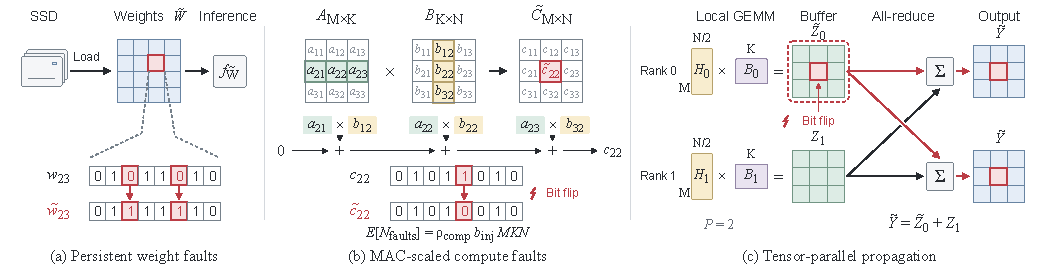
\includegraphics[width=\textwidth]{fault_models.pdf}
    \caption{\textbf{Model-visible fault abstractions supported by vLLM-FI.}
    Memory faults modify model weights during loading and persist throughout subsequent inference.
    Compute faults perturb intermediate results produced by matrix operations.
    Communication faults modify software-visible buffers associated with tensor-parallel collectives or pipeline-parallel transfers.}
    \label{fig:three_fault_models}
\end{figure*}


\subsubsection{Memory Faults}

Memory faults can corrupt data stored during LLM inference, including model weights, activations, and the KV cache. This work focuses on model weights because their long lifetime and repeated reuse allow corruption to affect many subsequent forward computations and decoding steps. A corrupted weight can therefore introduce persistent perturbations into inference and degrade downstream-task performance.

To evaluate this effect, vLLM-FI applies configurable bit flips to selected weight tensors as they are loaded into GPU memory. The modified values are retained and used in subsequent inference, allowing the evaluation workflow to measure their impact on model outputs. The loading stage serves as the injection point for establishing persistent weight corruption; the model does not restrict the physical occurrence of memory faults to model loading.

To determine the injection count, consider a weight tensor $\mathbf{W}$ containing $|\mathbf{W}|$ elements, each with a storage width of $b$ bits. Let $\rho_{\mathrm{mem}}$ denote the fault event rate per stored bit. The expected number of memory fault events is

\begin{equation}
    \lambda_{\mathrm{mem}}
    =
    |\mathbf{W}|b\rho_{\mathrm{mem}},
    \qquad
    N_{\mathrm{faults}}^{\mathrm{mem}}
    \sim
    \operatorname{Poisson}(\lambda_{\mathrm{mem}}).
    \label{eq:memory_exposure}
\end{equation}


\subsubsection{Compute Faults}

Compute faults model the effect of transient errors in arithmetic units on intermediate computation results \cite{ashraf2015understanding}. Existing model-level fault injection methods commonly estimate the number of compute faults according to the number of elements in an output tensor. However, the output size does not necessarily reflect the amount of computation required to produce that output.

For example, multiplying matrices with shapes $(a_1,a_2)$ and $(a_2,a_1)$ produces an output containing $a_1^2$ elements, but requires $a_1^2a_2$ multiply--accumulate operations. Increasing $a_2$ therefore increases the computational fault exposure without changing the number of output elements. This difference becomes more important for LLMs because of their large projection dimensions and the repeated execution of matrix operations during autoregressive decoding.

Following prior LLM reliability studies \cite{sun2025demystifying,sun2025ft2,xie2025realm}, vLLM-FI injects compute faults into the outputs of GEMM and related matrix operations. However, the number of faults is determined by the estimated multiply--accumulate workload rather than solely by the output-tensor size. Let $\mathcal{C}_{\mathrm{total}}$ be the estimated number of executed MAC operations and $b_{\mathrm{inj}}$ be the data width at the injection point. The compute exposure and the expected number of fault events are defined as

\begin{equation}
    \mathcal{E}_{\mathrm{comp}}
    =
    \mathcal{C}_{\mathrm{total}}b_{\mathrm{inj}},
    \qquad
    \lambda_{\mathrm{comp}}
    =
    \rho_{\mathrm{comp}}\mathcal{E}_{\mathrm{comp}},
    \label{eq:compute_exposure}
\end{equation}

\begin{equation}
    N_{\mathrm{faults}}^{\mathrm{comp}}
    \sim
    \operatorname{Poisson}(\lambda_{\mathrm{comp}}),
    \label{eq:compute_poisson}
\end{equation}

where $\rho_{\mathrm{comp}}$ denotes the compute-fault event rate per exposed bit operation.

Algorithm~\ref{alg:mac_estimation} summarizes the runtime MAC estimation procedure. Linear projections use their executed batch size, input dimension, and output dimension. Fused modules, such as \texttt{gate\_up\_proj}, are treated according to the dimensions of the fused runtime operator. Attention computation is estimated using the sequence metadata provided by vLLM, allowing the framework to distinguish prefill from decode and to account for the effective number of query--key pairs under causal attention. The current model excludes non-MAC operations such as Softmax, normalization, rotary position encoding, and data movement.

\begin{algorithm}[t]
\footnotesize
\DontPrintSemicolon
\SetAlgoVlined
\SetInd{0.35em}{0.75em}
\SetAlgoNlRelativeSize{-1}
\caption{Runtime MAC Estimation}
\label{alg:mac_estimation}
\KwIn{Projection shapes $\mathcal{P}$; query offsets $\mathbf{s}$; context lengths $\boldsymbol{\ell}$; query-head count $N_q$; head dimension $D_h$}
\KwOut{Estimated MAC count $\mathcal{C}_{\mathrm{total}}$}

$\mathcal{C}_{\mathrm{proj}} \leftarrow 0$;

\ForEach{$(N,D_{\mathrm{in}},D_{\mathrm{out}}) \in \mathcal{P}$}{
    $\mathcal{C}_{\mathrm{proj}}
    \leftarrow
    \mathcal{C}_{\mathrm{proj}}
    +
    ND_{\mathrm{in}}D_{\mathrm{out}}$;
}

$\mathcal{C}_{\mathrm{attn}} \leftarrow 0$;

\For{$i \leftarrow 0$ \KwTo $|\boldsymbol{\ell}|-1$}{
    $L_q \leftarrow \mathbf{s}[i+1]-\mathbf{s}[i]$;

    $L_{\mathrm{kv}} \leftarrow \boldsymbol{\ell}[i]$;

    \eIf{$L_q>1$}{
        $N_{\mathrm{eff}}
        \leftarrow
        L_q\left(
        L_{\mathrm{kv}}
        -
        \frac{L_q-1}{2}
        \right)$;
    }{
        $N_{\mathrm{eff}}
        \leftarrow
        L_qL_{\mathrm{kv}}$;
    }

    $\mathcal{C}_{\mathrm{attn}}
    \leftarrow
    \mathcal{C}_{\mathrm{attn}}
    +
    2N_qN_{\mathrm{eff}}D_h$;
}

$\mathcal{C}_{\mathrm{total}}
\leftarrow
\mathcal{C}_{\mathrm{proj}}
+
\mathcal{C}_{\mathrm{attn}}$;

\Return{$\mathcal{C}_{\mathrm{total}}$};
\end{algorithm}


\subsubsection{Communication Faults}

Communication faults model errors affecting data exchanged between devices during distributed inference. vLLM-FI targets software-visible communication buffers in both tensor-parallel and pipeline-parallel execution. For tensor parallelism, faults are injected into buffers associated with collective operations such as All-Reduce. For pipeline parallelism, faults are injected into activation buffers transferred between adjacent pipeline stages.

At a selected communication location, let $\mathbf{B}$ denote the communication buffer, $|\mathbf{B}|$ the number of elements in that buffer, $b$ the number of bits per element, and $\rho_{\mathrm{comm}}$ the communication-fault event rate. The number of injected communication faults is sampled as

\begin{equation}
    \lambda_{\mathrm{comm}}
    =
    |\mathbf{B}|b\rho_{\mathrm{comm}},
    \qquad
    N_{\mathrm{faults}}^{\mathrm{comm}}
    \sim
    \operatorname{Poisson}(\lambda_{\mathrm{comm}}).
    \label{eq:comm_exposure}
\end{equation}

The selected bits are modified before the corresponding collective operation or pipeline-stage transfer. The corrupted buffer therefore participates in subsequent communication and computation, allowing the resulting error to propagate across devices. This abstraction models corruption that is visible in the software communication path. Low-level link protocols, retransmission mechanisms, and internal interconnect behavior remain outside the scope of vLLM-FI.


\subsection{vLLM-Native Fault Injection and Evaluation}
\label{subsec:runtime_injection}

Introducing an independent fault configuration into vLLM is non-trivial. To reach the actual injection locations, a newly defined configuration must pass through the Engine, Executor, Worker processes, ModelRunner, and runtime layer implementations. vLLM-FI addresses this problem by implementing \textit{FaultConfig} as a sub-configuration of \textit{VllmConfig}. The fault configuration can therefore reuse the native vLLM configuration-propagation path and reach the corresponding injection locations inside each Worker. Each Worker evaluates the fault-activation settings in \textit{FaultConfig} against its current device, rank, pipeline stage, model module, fault type, and execution conditions, and activates the corresponding injector when the configured conditions are satisfied. In this way, \textit{FaultConfig} provides configuration-level support for distributed fault injection without introducing an independent cross-process control path.

Weight fault injection additionally requires resolving the runtime parameter held by each Worker. If injection were performed by traversing the entire model after model loading, the target specified in the fault configuration would have to be remapped to the runtime parameters held by different Workers under the selected parallel configuration. To avoid implementing this additional mapping procedure, vLLM-FI embeds weight fault injection into the weight-loading methods of vLLM linear layers. At this location, the target model layer and the parameter currently being loaded by the Worker are directly available. Without tensor parallelism, the injector operates on the complete loaded parameter. Under tensor parallelism, it operates on the weight shard selected for the current rank. Under pipeline parallelism, the weight-loading method is executed only for the model layers assigned to the current pipeline stage. Quantized weights, including packed \texttt{qweight} parameters, follow the same injection path and are distinguished through an additional check of the parameter name and storage representation.

Unlike weight faults, compute and communication faults occur during runtime inference rather than during model loading. vLLM-FI therefore places their injection sites in the forward execution paths of the corresponding runtime layers. A compute fault is triggered after the selected matrix operation produces its output. A communication fault modifies the corresponding communication buffer before a tensor-parallel collective or a pipeline-stage transfer. Because these injection mechanisms execute inside the Worker, they directly operate on the runtime tensors produced under the current device and parallel context. Together with the distributed activation settings provided by \textit{FaultConfig}, the runtime injection mechanisms support tensor parallelism, pipeline parallelism, and their combined configurations. Placing the injection sites in shared runtime layer definitions also allows the same mechanism to be reused across supported model architectures.

Reliability evaluation across different models, datasets, and inference configurations otherwise requires repeated implementation of dataset loading, model invocation, output processing, and task-specific metric calculation. To reduce this repeated work, vLLM-FI adapts \texttt{lm-evaluation-harness} to support \textit{FaultConfig}. The modified interface passes \textit{FaultConfig}, together with the existing vLLM parameters, to the vLLM backend. It constructs benchmark inputs, executes inference under the specified fault configuration, collects the fault-affected outputs, and computes the native metrics of the selected downstream task. This integration provides an end-to-end workflow from distributed fault injection to standardized task-level reliability evaluation.


\subsection{GPU-Resident In-Place Bit-Flip Operator}
\label{subsec:cuda_operator}

Existing model-level fault injection tools for CNNs and conventional DNNs generally prioritize portable and extensible implementations based on PyTorch-level operations \cite{mahmoud2020pytorchfi,huang2024mrfi}. Their typical experiments inject only one or a small number of faults during each forward pass. Under such workloads, the additional injection overhead is relatively limited, and the performance benefit of developing and maintaining a dedicated CUDA operator is therefore less significant.

This design trade-off changes for LLM fault injection. Autoregressive generation repeatedly executes model layers across multiple decoding steps, causing runtime injection sites to be triggered many times. Moreover, vLLM-FI determines the number of fault events according to the configured error rate and compute exposure, such that more faults must be processed as the target workload or error rate increases. With CPU-assisted bit modification, host--device transfers and synchronization are repeatedly introduced across model layers and decoding steps, while a larger number of faults also increases the transferred data volume and host-side bit-manipulation workload. As shown in Fig.~\ref{fig:controlled_injection_runtime}, the runtime difference between CPU-assisted and CUDA-based injection is relatively small at low error rates but grows rapidly as the error rate and the number of injected faults increase. GPU-resident batched in-place modification therefore changes from an optional optimization for conventional workloads into a practical requirement for efficient LLM fault injection.

To eliminate this CPU round trip, vLLM-FI implements a custom CUDA bit-flip operator that directly modifies target tensors residing in GPU memory. Given a target tensor and the fault injection parameters, the operator performs target-position selection, bit-mask construction, and binary-data modification on the GPU without copying the selected values to the CPU. This design confines the data manipulation introduced by fault injection to the GPU and allows multiple fault events within an injection call to be processed in parallel.

Moving bit flipping to the GPU also requires adapting the injection procedure to different data representations. Full-precision and quantized data types have different storage widths and encoding layouts and therefore cannot be modified using a single uniform bit-manipulation procedure. vLLM-FI implements data-type-specific bit operations for each supported representation.

For each fault event, the CUDA operator independently samples an element from the target tensor and selects one or two distinct bit positions permitted by the configured bit-selection policy. It then constructs an XOR mask from the selected positions and applies the mask to the underlying binary representation of the target element.

The eligible bit positions are determined jointly by the tensor data type and the configured bit-selection policy. Full-width injection supports FP64, FP32, FP16, BF16, INT8, UINT8, INT16, INT32, INT64, FP8 E5M2, and FP8 E4M3FN. For FP16, BF16, and FP8 values, field-specific injection can further restrict faults to the sign, exponent, or mantissa field. Through type-specific dispatch over the underlying storage representation, the same operator can directly process full-precision weights and activations, quantized weights, and other intermediate representations without first converting them to a common CPU format.

% \section{vLLM-FI Framework}
% \label{sec:framework}

% This section presents the design and implementation of vLLM-FI. It focuses on how the tool performs configurable fault injection on the native vLLM execution path. We first describe the constraints imposed by the multi-process runtime and the overall architecture. The remaining subsections present fault models, cross-process configuration propagation, runtime target selection, GPU-resident bit flipping, and automated reliability evaluation.

% \subsection{Design Goals and System Architecture}
% \label{subsec:architecture}

% vLLM improves inference throughput and GPU memory utilization through continuous batching, PagedAttention-based KV-cache management, optimized computation kernels, and distributed parallel execution \cite{kwon2023efficient}. However, the runtime architecture supporting these optimizations complicates conventional hook-based fault injection. Unlike a typical PyTorch program, which stores the model object in a single process, vLLM executes models in Worker processes launched by a scheduling process. Consequently, model instances and layer objects reside inside the Workers and are not directly accessible from the entry process. External forward hooks therefore cannot reliably locate or modify a target layer. Distributed execution further partitions parameters and intermediate results across ranks. vLLM-FI must therefore propagate fault configurations across process boundaries and perform injection inside the appropriate Worker at the correct rank and runtime location.

% vLLM-FI addresses these constraints through a configuration-driven injection path integrated into the native vLLM runtime. For each experiment, the system receives a set of inference requests, a vLLM execution configuration, and a \textit{Fault Config}. The vLLM execution configuration specifies the model, quantization method, parallel configuration, and inference parameters, whereas the \textit{Fault Config} specifies the fault type, injection target, and injection strength. During execution, the fault configuration is propagated to the Workers, where vLLM-FI applies controlled perturbations to selected model weights, operator outputs, or communication buffers. The resulting inference outputs retain the format expected by downstream task evaluators.

% Three goals guide this architecture: configuration simplicity, efficient injection, and precise runtime targeting. First, vLLM-FI manages the \textit{Fault Config} together with the native vLLM execution parameters and automatically handles its propagation across processes. Second, it modifies GPU-resident target tensors in place, avoiding CPU copies and host--device transfers introduced solely by fault injection. Third, it resolves injection targets using the runtime representations and execution locations employed by vLLM, including quantized tensors, fused operators, and rank-local data. These extensions do not alter model partitioning, Worker launch, device placement, or scheduling, which remain under the control of vLLM.

% \begin{figure*}[t]
%     \centering
%     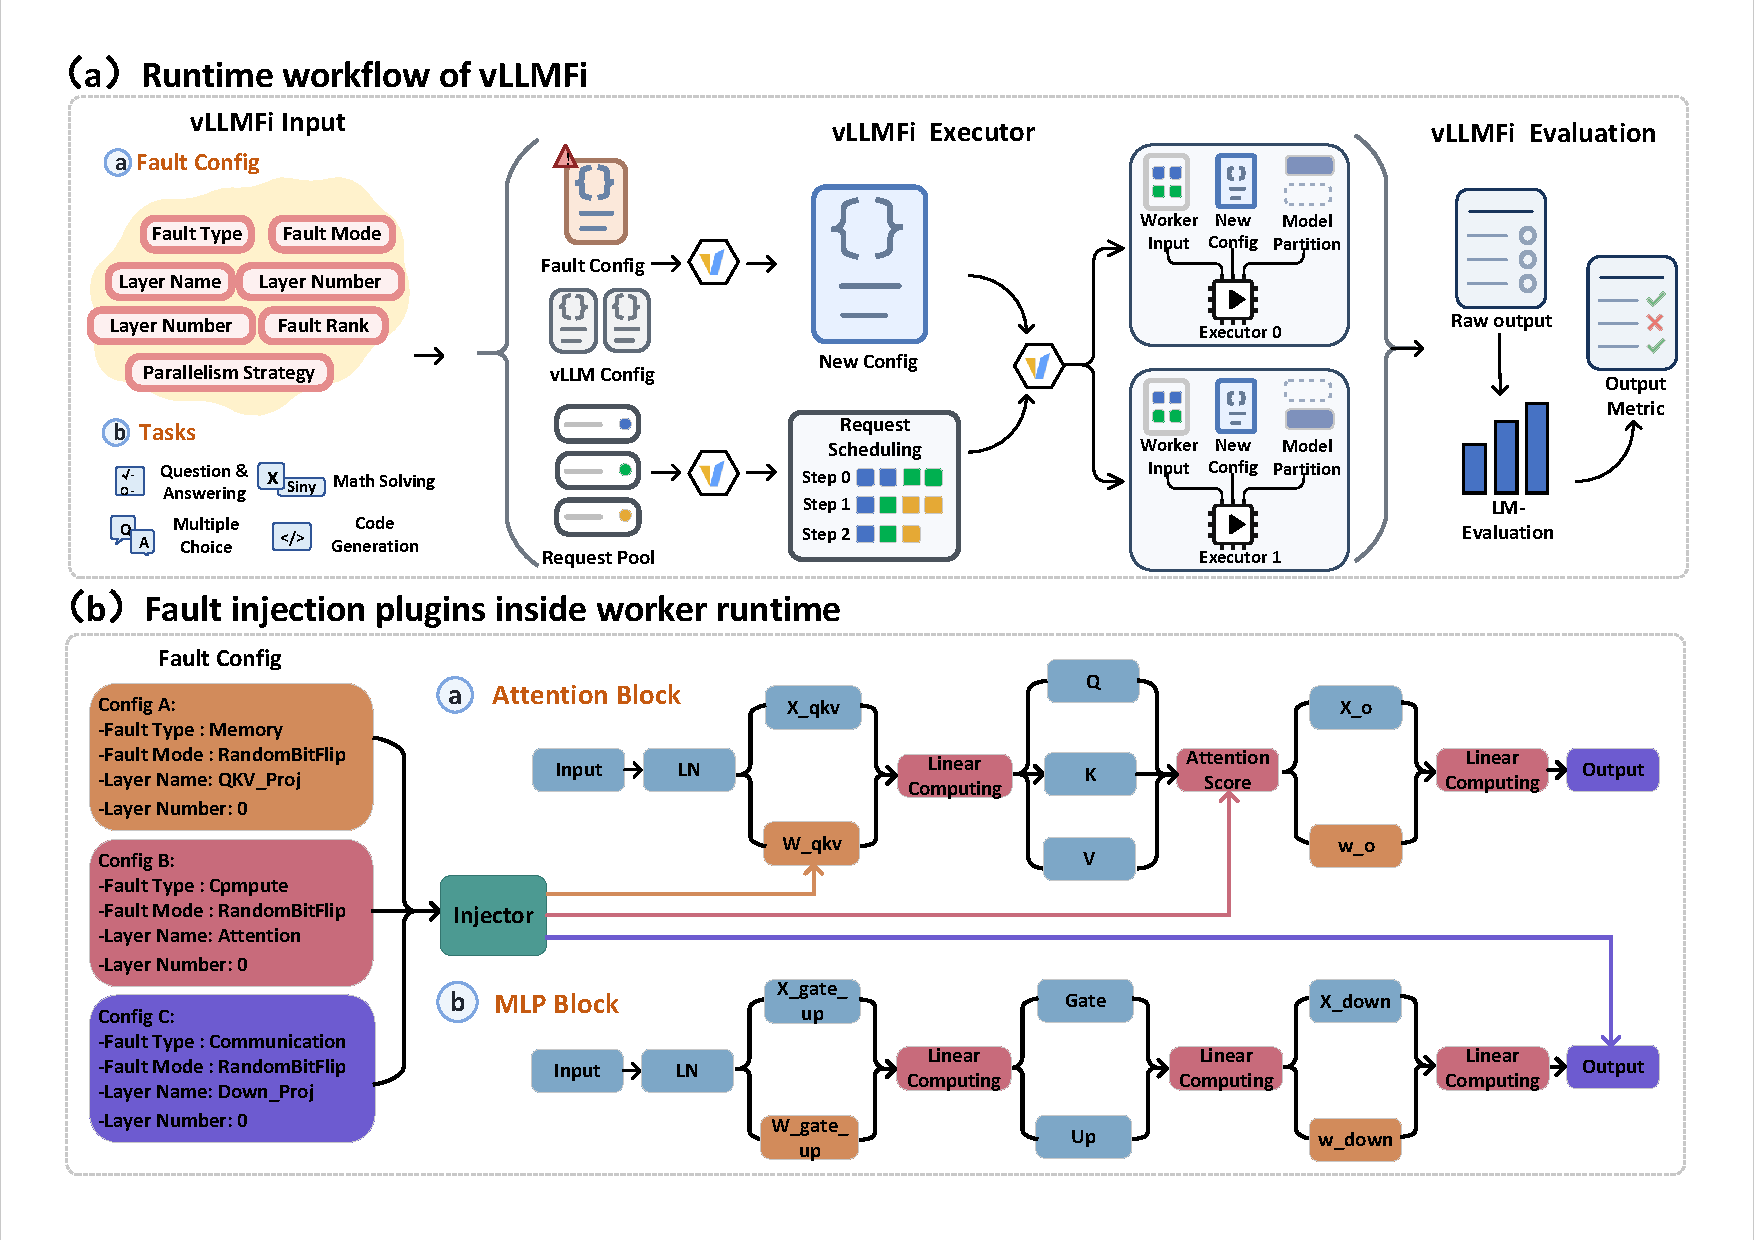
\includegraphics[width=0.82\textwidth]{vLLMFI.pdf}
%     \caption{\textbf{Overview of the vLLM-FI architecture and execution workflow.}
%     vLLM schedules inference requests from the evaluation dataset, while Fault Config is integrated with the native configuration and propagated to the Workers. Worker-side injectors perturb selected GPU-resident tensors during inference, and \texttt{lm-evaluation} evaluates the resulting outputs.}
%     \label{fig:vllmfi_architecture}
% \end{figure*}

% Figure~\ref{fig:vllmfi_architecture} illustrates the configuration-driven architecture and execution workflow of vLLM-FI. The evaluation dataset and Fault Config are provided as system inputs, while vLLM schedules the inference requests generated from the dataset. Fault Config is integrated with the native vLLM execution configuration to form a unified runtime configuration, which is then propagated to the Workers through the Executor. During model inference, each Worker activates the appropriate fault injector according to the fault type, injection target, and injection strength specified in Fault Config. The fault-affected model outputs are subsequently returned to lm-evaluation, which evaluates the injection results using the task-specific metrics associated with the dataset.

% \subsection{Fault Models and Injection-Strength Modeling}
% \label{subsec:fault_models}

% vLLM-FI defines memory, compute, and communication faults on model weights, operator results, and communication buffers. The framework supports fixed-count and bit error rate modes.Fixed-count mode specifies the number of fault events. BER mode derives the Poisson parameter $\lambda$ from the exposure of the target object. The following subsections define the exposure and event count for each fault model.

% \begin{figure*}[t]
%     \centering
%     \subfloat[Memory fault during weight loading.\label{fig:fault_memory}]{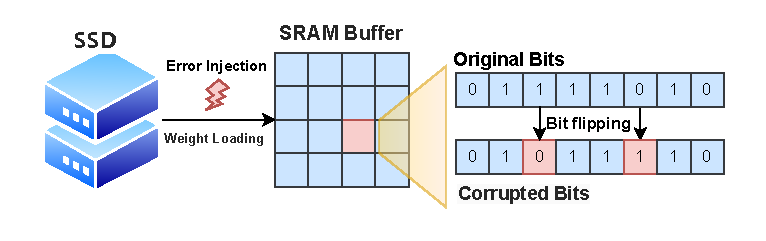
\includegraphics[width=0.30\textwidth]{memory_error.drawio.pdf}}
%     \hfill
%     \subfloat[Compute fault in an operator result.\label{fig:fault_compute}]{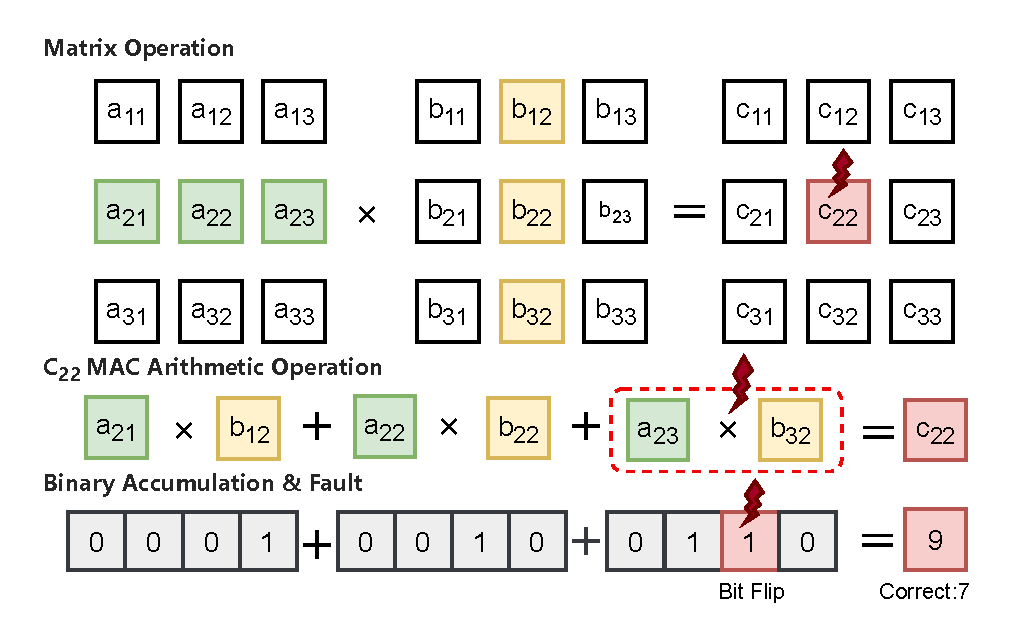
\includegraphics[width=0.30\textwidth]{compute_error.drawio.pdf}}
%     \hfill
%     \subfloat[Communication fault before a collective.\label{fig:fault_comm}]{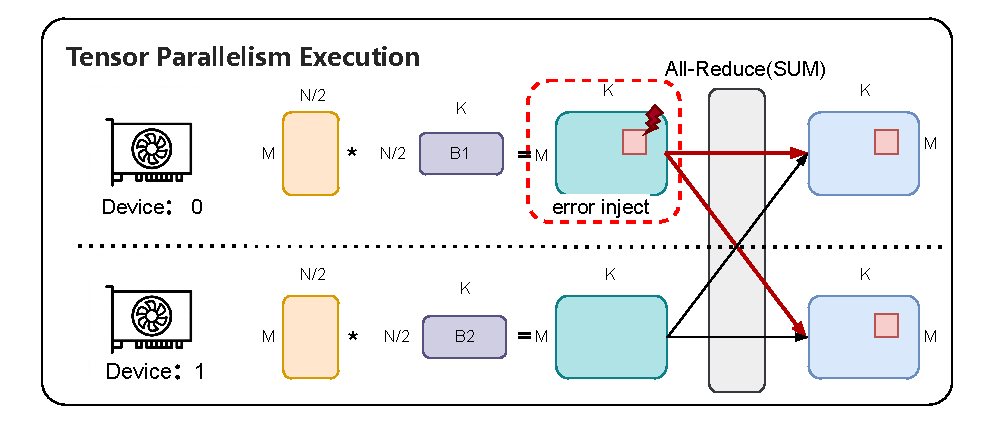
\includegraphics[width=0.30\textwidth]{communication_error_v2.drawio.pdf}}
%     \caption{Model-visible fault abstractions in vLLM-FI. A weight perturbation persists after loading. A compute perturbation changes an intermediate result. A communication perturbation is applied to a local buffer before collective communication and may propagate through data exchange or aggregation.}
%     \label{fig:three_fault_models}
% \end{figure*}

% \subsubsection{Memory Faults}

% Memory faults model weight corruption during storage or loading. Error-correcting code can detect or correct many single-bit errors. Uncorrectable multi-bit errors may still cause silent data corruption \cite{hsiao2023silent,papadimitriou2021demystifying,jiao2025large}. vLLM-FI injects random double-bit flips while weights enter the GPU execution path. A modified weight remains corrupted during subsequent forward computations and autoregressive decoding.

% For a weight tensor $\mathbf{W}$ with $|\mathbf{W}|$ elements and a storage width of $b$ bits per element, let $\rho_{\mathrm{mem}}$ be the fault-event rate per stored bit. The fault count is
% \begin{equation}
%     \lambda_{\mathrm{mem}}=|\mathbf{W}|b\rho_{\mathrm{mem}},
%     \qquad
%     N_{\mathrm{faults}}^{\mathrm{mem}}
%     \sim \operatorname{Poisson}(\lambda_{\mathrm{mem}}).
%     \label{eq:memory_exposure}
% \end{equation}

% \subsubsection{Compute Faults}

% Compute faults model the effect of transient errors in arithmetic units on intermediate results \cite{ashraf2015understanding}. Following prior LLM reliability studies \cite{sun2025demystifying,sun2025ft2,xie2025realm}, vLLM-FI maps them to bit perturbations in GEMM and related matrix-computation outputs.

% Compute exposure is defined by the multiply--accumulate (MAC) workload represented by the target operators. Let $\mathcal{C}_{\mathrm{total}}$ be the estimated MAC count and $b_{\mathrm{inj}}$ the data width at the injection point. The bit-level compute exposure and expected event count are
% \begin{equation}
%     \mathcal{E}_{\mathrm{comp}}=\mathcal{C}_{\mathrm{total}}b_{\mathrm{inj}},
%     \qquad
%     \lambda_{\mathrm{comp}}=\rho_{\mathrm{comp}}\mathcal{E}_{\mathrm{comp}},
%     \label{eq:compute_exposure}
% \end{equation}
% \begin{equation}
%     N_{\mathrm{faults}}^{\mathrm{comp}}
%     \sim \operatorname{Poisson}(\lambda_{\mathrm{comp}}).
%     \label{eq:compute_poisson}
% \end{equation}

% Algorithm~\ref{alg:mac_estimation} summarizes the runtime MAC estimate. Linear projections use their executed input and output dimensions. Fused modules, such as \texttt{gate\_up\_proj}, use the dimensions of the fused runtime operator. Attention uses sequence metadata supplied by vLLM to distinguish prefill from decode. The current estimate excludes non-MAC operations, including Softmax, normalization, rotary position encoding, and data movement.

% % This algorithm is intentionally single-column.
% \begin{algorithm}[t]
% \footnotesize
% \DontPrintSemicolon
% \SetAlgoVlined
% \SetInd{0.35em}{0.75em}
% \SetAlgoNlRelativeSize{-1}
% \caption{Runtime MAC Estimation}
% \label{alg:mac_estimation}
% \KwIn{Projection shapes $\mathcal{P}$; query offsets $\mathbf{s}$; context lengths $\boldsymbol{\ell}$; query-head count $N_q$; head dimension $D_h$}
% \KwOut{Estimated MAC count $\mathcal{C}_{\mathrm{total}}$}
% $\mathcal{C}_{\mathrm{proj}} \leftarrow 0$;
% \ForEach{$(N,D_{\mathrm{in}},D_{\mathrm{out}}) \in \mathcal{P}$}{
%     $\mathcal{C}_{\mathrm{proj}} \leftarrow \mathcal{C}_{\mathrm{proj}}+ND_{\mathrm{in}}D_{\mathrm{out}}$;
% }
% $\mathcal{C}_{\mathrm{attn}} \leftarrow 0$;
% \For{$i \leftarrow 0$ \KwTo $|\boldsymbol{\ell}|-1$}{
%     $L_q \leftarrow \mathbf{s}[i+1]-\mathbf{s}[i]$;
%     $L_{\mathrm{kv}} \leftarrow \boldsymbol{\ell}[i]$;
%     \eIf{$L_q>1$}{
%         $N_{\mathrm{eff}} \leftarrow L_q\left(L_{\mathrm{kv}}-\frac{L_q-1}{2}\right)$;
%     }{
%         $N_{\mathrm{eff}} \leftarrow L_qL_{\mathrm{kv}}$;
%     }
%     $\mathcal{C}_{\mathrm{attn}} \leftarrow \mathcal{C}_{\mathrm{attn}}+2N_qN_{\mathrm{eff}}D_h$;
% }
% $\mathcal{C}_{\mathrm{total}} \leftarrow \mathcal{C}_{\mathrm{proj}}+\mathcal{C}_{\mathrm{attn}}$;
% \Return{$\mathcal{C}_{\mathrm{total}}$};
% \end{algorithm}

% \subsubsection{Communication Faults}

% Communication faults model errors during data exchange in multi-device inference. vLLM-FI flips bits in a local communication buffer before a collective call. Corrupted data then participates in operations such as All-Reduce and may propagate to other ranks.

% Communication exposure is derived from the transferred data volume. Consider a Ring All-Reduce with tensor-parallel size $P$ and a communication tensor containing $N_{\mathrm{elem}}$ elements. Its Reduce-Scatter and All-Gather phases produce the following per-rank element volume:
% \begin{equation}
%     V_{\mathrm{comm}}=\frac{2(P-1)}{P}N_{\mathrm{elem}}.
%     \label{eq:comm_volume}
% \end{equation}
% For a communication width of $b$ bits and a target rate $\rho_{\mathrm{comm}}$, vLLM-FI samples
% \begin{equation}
%     \lambda_{\mathrm{comm}}=V_{\mathrm{comm}}b\rho_{\mathrm{comm}},
%     \qquad
%     N_{\mathrm{faults}}^{\mathrm{comm}}
%     \sim \operatorname{Poisson}(\lambda_{\mathrm{comm}}).
%     \label{eq:comm_exposure}
% \end{equation}
% This model separates communication-path exposure from an equal-sized local tensor perturbation. It captures the software-visible buffer corruption. Link protocols, retransmission, and internal interconnect behavior remain outside its scope.

% \subsection{Configuration-Driven Runtime Injection}
% \label{subsec:runtime_injection}

% Fault Config extends the native vLLM execution configuration with controlled fault-injection metadata. It records the fault type, fault mode, target rank, injection strength and random seed. The evaluation dataset and Fault Config are provided to vLLM-FI as system inputs. vLLM schedules the inference requests derived from the dataset, while vLLM-FI integrates Fault Config with the native execution settings to form a unified runtime configuration. The Executor then propagates this configuration to the Workers.

% Within each Worker, vLLM-FI registers candidate injection sites along the weight-loading, operator-computation, and collective-communication paths. At each candidate site, the Worker checks the current module, execution stage, and local rank against Fault Config. When all conditions match, the Worker passes the target tensor and injection parameters to the custom CUDA bit-flip operator, which modifies the selected GPU-resident tensor in place.

% Rank selection supports a single rank, a list of ranks, or all ranks. Each Worker compares its local rank with the configured target set. Single-rank mode enables injection only in the selected Worker, while multi-rank mode enables injection in the listed Workers. All-rank mode permits injection in every Worker that satisfies the configured module and execution-stage conditions.

% The mechanism operates within the native parallel context created by vLLM and does not alter model partitioning, device placement, or scheduling. Under tensor parallelism, a matching Worker modifies the local parameter shard, intermediate tensor, or communication buffer that it owns. Under pipeline parallelism, injection is activated only in the stage that executes the target layer and satisfies the rank condition.

% For communication faults, the injection scope covers all inter-GPU communication sites, including collective communication within tensor-parallel layers and activation transfers at pipeline-stage boundaries. Within each communicated tensor, fault locations are sampled according to the configured bit error rate. After inference, the fault-affected outputs are returned to \texttt{lm-evaluation} for task-specific evaluation.
% \subsection{GPU-Resident In-Place Bit-Flip Operator}
% \label{subsec:cuda_operator}

% vLLM-FI uses a custom CUDA operator to modify selected GPU-resident tensors in place. The operator receives a tensor pointer and the injection parameters, and directly modifies the underlying binary storage without creating a CPU copy.

% For each fault event, the operator samples a tensor element and selects one or two distinct bit positions permitted by the configured policy. It constructs an XOR mask from the selected positions and applies the mask to the stored binary representation of the element. The eligible bit positions are determined by the tensor data type and the bit-selection policy. Full-width mode supports FP64, FP32, FP16, BF16, INT8, UINT8, INT16, INT32, INT64 , FP8 E5M2 and FP8 E4M3FN. Field-specific mode restricts faults in FP16, BF16, and FP8 values to the sign, exponent, or mantissa fields.

% Updates are performed using atomic XOR operations. For 32-bit and 64-bit storage words, the operator applies the mask directly to the corresponding word. Since CUDA does not provide native atomic XOR operations for 8-bit or 16-bit values, vLLM-FI maps each target value to its enclosing aligned 32-bit word. It then shifts the mask according to the byte or half-word offset and performs a 32-bit atomic XOR operation. This procedure preserves the remaining bits in the storage word and prevents lost updates when multiple threads concurrently access the same word.
% The kernel assigns scheduled fault events to CUDA threads. The element and bit positions for each event are determined by a base random seed and the thread index. The kernel executes on the caller-provided CUDA stream without introducing explicit device-wide synchronization. Identical configurations, random seeds, and execution conditions reproduce the same injection positions. Section 5 evaluates the end-to-end runtime overhead.

% \subsection{Automated End-to-End Reliability Evaluation}
% \label{subsec:evaluation_loop}

% Fault injection produces perturbed outputs. A complete reliability study must also load tasks, construct inputs, run inference, score outputs, and aggregate results. Separate scripts for these steps increase the effort required to add a task or fault configuration. vLLM-FI integrates with \texttt{lm-evaluation-harness} to expose one evaluation workflow.

% Users select the model, downstream task, vLLM settings, and Fault Config through a common command-line entry. The system initializes the model, propagates the fault configuration, triggers runtime injection, collects outputs, and invokes the task evaluator. Changing the fault model, target, or task requires configuration changes rather than new model-loading, trigger, or scoring code.

% The task evaluator first produces the native benchmark metric. The result-processing stage aggregates repeated runs and computes normalized values against a fault-free baseline. This configuration-driven loop simplifies batch experiments and records the information required for reproduction. Section~\ref{sec:experimental_setup} defines the common workloads and evaluation protocol.

\section{Experimental Setup}
\label{sec:experimental_setup}

This section reports the common setup used to validate vLLM-FI and evaluate LLM inference reliability.

\subsection{Experimental Platform and Workloads}
\label{subsec:platform_workloads}

Experiments run on a server with eight NVIDIA A100-SXM4-80GB GPUs. Distributed experiments use four GPUs. The software stack consists of Ubuntu 20.04.6, Python 3.12.11, PyTorch 2.6.0+cu124, CUDA 12.2, NCCL 2.21.5, vLLM 0.8.5 \cite{kwon2023efficient}, and \texttt{lm-evaluation-harness} 0.4.9.2. All tasks use fixed random seeds. Generative tasks disable sampling and use deterministic decoding.

LLaMA-3.1-8B \cite{grattafiori2024llama} is the primary model for tool validation, task-level reliability analysis, and quantization experiments.The quantization study evaluates AWQ W4A16 \cite{lin2024awq}, GPTQ W4A16, GPTQ W8A16 \cite{frantar2022gptq}, and FP8 W8A16 variants from the same model family. Communication and model-parallel experiments also include Qwen-2.5-7B \cite{yang2024qwen25} and Mistral-7B \cite{jiang2023mistral}.

The workload suite covers knowledge questions, commonsense reasoning, multidisciplinary knowledge, mathematical reasoning, text summarization, and code generation. ARC-Challenge, HellaSwag, MMLU, and GSM8K use the 100-sample configurations supplied by tinyBenchmarks \cite{polo2024tinybenchmarks} to control the cost of repeated fault-injection runs. Table~\ref{tab:workloads} lists the tasks and native metrics.

% This table is intentionally single-column and avoids resizebox/scalebox.
\begin{table}[t]
\caption{Downstream Workloads and Evaluation Metrics}
\label{tab:workloads}
\centering
\footnotesize
\renewcommand{\arraystretch}{1.10}
\setlength{\tabcolsep}{3.2pt}
\begin{tabularx}{\columnwidth}{@{}>{\raggedright\arraybackslash}X >{\centering\arraybackslash}p{0.43in} >{\centering\arraybackslash}p{0.38in} >{\raggedright\arraybackslash}p{0.78in}@{}}
\toprule
\textbf{Task} & \textbf{Samples} & \textbf{Shots} & \textbf{Metric} \\
\midrule
\multicolumn{4}{@{}l}{\itshape Multiple-choice tasks} \\
tinyARC \cite{clark2018think}              & 100   & 25 & Norm. accuracy \\
tinyHellaSwag \cite{zellers2019hellaswag} & 100   & 10 & Norm. accuracy \\
tinyMMLU \cite{hendrycks2020measuring}    & 100   & 0  & Norm. accuracy \\
\addlinespace[2pt]
\multicolumn{4}{@{}l}{\itshape Autoregressive generation tasks} \\
tinyGSM8K \cite{cobbe2021training}        & 100   & 5  & Exact Match \\
CNN/DailyMail \cite{hermann2015teaching}  & 1,149 & 0  & ROUGE-1 \cite{lin2004rouge} \\
HumanEval \cite{chen2021evaluating}       & 164   & 0  & Pass@1 \\
\bottomrule
\end{tabularx}
\end{table}

\subsection{Evaluation Protocol}
\label{subsec:evaluation_protocol}

The fault-free performance of each task and model configuration serves as its baseline. Let $m_{\mathrm{clean}}$ denote this baseline and $m_{\mathrm{fault}}^{(i)}$ the metric from fault-injection run $i$. Performance retention is
\begin{equation}
    R^{(i)}=\frac{m_{\mathrm{fault}}^{(i)}}{m_{\mathrm{clean}}}.
    \label{eq:performance_retention}
\end{equation}
A value of $R=1$ matches the fault-free baseline. A smaller value indicates greater degradation. Each quantized configuration uses its own fault-free result as the baseline.

Section~5 presents tool correctness and runtime cost, memory and compute faults across tasks, quantized representations, communication paths, and TP/PP rank selection. Each result subsection begins with its experiment-specific fault settings and controls, followed by quantitative results and analysis.

\section{Experimental Evaluation}
\label{sec:experimental_evaluation}

This section evaluates the effectiveness of vLLM-FI and the reliability of large language models under different fault conditions. We first describe the experimental setup and then calibrate the fault injection behavior of vLLM-FI against MRFI. We then analyze the effects of compute and memory faults across downstream tasks and evaluate how weight-only quantization affects sensitivity to memory faults. Finally, we examine reliability differences in distributed inference, including those associated with communication strategies and model-parallel configurations. Unless otherwise specified, the fault injection scope covers all model layers. For device-specific injection in model-parallel experiments, the scope covers all model layers or layer partitions assigned to the selected GPU.

\section{Experimental Setup}
\label{sec:experimental_setup}

This section reports the common setup used to validate vLLM-FI and evaluate LLM inference reliability.

\subsection{Experimental Platform and Workloads}
\label{subsec:platform_workloads}

Experiments run on a server with eight NVIDIA A100-SXM4-80GB GPUs. Distributed experiments use four GPUs. The software stack consists of Ubuntu 20.04.6, Python 3.12.11, PyTorch 2.6.0+cu124, CUDA 12.2, NCCL 2.21.5, vLLM 0.8.5 \cite{kwon2023efficient}, and \texttt{lm-evaluation-harness} 0.4.9.2. All tasks use fixed random seeds. Generative tasks disable sampling and use deterministic decoding.

LLaMA-3.1-8B \cite{grattafiori2024llama} is the primary model for tool validation, task-level reliability analysis, and quantization experiments.The quantization study evaluates AWQ W4A16 \cite{lin2024awq}, GPTQ W4A16, GPTQ W8A16 \cite{frantar2022gptq}, and FP8 W8A16 variants from the same model family. Communication and model-parallel experiments also include Qwen-2.5-7B \cite{yang2024qwen25} and Mistral-7B \cite{jiang2023mistral}.

The workload suite covers knowledge questions, commonsense reasoning, multidisciplinary knowledge, mathematical reasoning, text summarization, and code generation. ARC-Challenge, HellaSwag, MMLU, and GSM8K use the 100-sample configurations supplied by tinyBenchmarks \cite{polo2024tinybenchmarks} to control the cost of repeated fault-injection runs. Table~\ref{tab:workloads} lists the tasks and native metrics.

% This table is intentionally single-column and avoids resizebox/scalebox.
\begin{table}[t]
\caption{Downstream Workloads and Evaluation Metrics}
\label{tab:workloads}
\centering
\footnotesize
\renewcommand{\arraystretch}{1.10}
\setlength{\tabcolsep}{3.2pt}
\begin{tabularx}{\columnwidth}{@{}>{\raggedright\arraybackslash}X >{\centering\arraybackslash}p{0.43in} >{\centering\arraybackslash}p{0.38in} >{\raggedright\arraybackslash}p{0.78in}@{}}
\toprule
\textbf{Task} & \textbf{Samples} & \textbf{Shots} & \textbf{Metric} \\
\midrule
\multicolumn{4}{@{}l}{\itshape Multiple-choice tasks} \\
tinyARC \cite{clark2018think}              & 100   & 25 & Norm. accuracy \\
tinyHellaSwag \cite{zellers2019hellaswag} & 100   & 10 & Norm. accuracy \\
tinyMMLU \cite{hendrycks2020measuring}    & 100   & 0  & Norm. accuracy \\
\addlinespace[2pt]
\multicolumn{4}{@{}l}{\itshape Autoregressive generation tasks} \\
tinyGSM8K \cite{cobbe2021training}        & 100   & 5  & Exact Match \\
CNN/DailyMail \cite{hermann2015teaching}  & 1,149 & 0  & ROUGE-1 \cite{lin2004rouge} \\
HumanEval \cite{chen2021evaluating}       & 164   & 0  & Pass@1 \\
\bottomrule
\end{tabularx}
\end{table}

\subsection{Evaluation Protocol}
\label{subsec:evaluation_protocol}

The fault-free performance of each task and model configuration serves as its baseline. Let $m_{\mathrm{clean}}$ denote this baseline and $m_{\mathrm{fault}}^{(i)}$ the metric from fault-injection run $i$. Performance retention is
\begin{equation}
    R^{(i)}=\frac{m_{\mathrm{fault}}^{(i)}}{m_{\mathrm{clean}}}.
    \label{eq:performance_retention}
\end{equation}
A value of $R=1$ matches the fault-free baseline. A smaller value indicates greater degradation. Each quantized configuration uses its own fault-free result as the baseline.

Section~5 presents tool correctness and runtime cost, memory and compute faults across tasks, quantized representations, communication paths, and TP/PP rank selection. Each result subsection begins with its experiment-specific fault settings and controls, followed by quantitative results and analysis.


\subsection{Tool Validation and Calibration}
\begin{figure}[t]
    \centering
    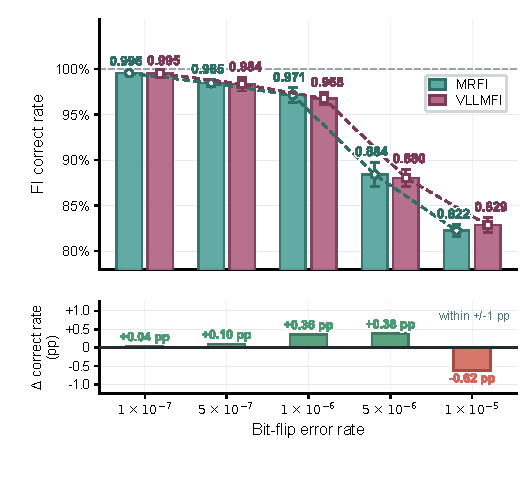
\includegraphics[width=\columnwidth]{fig_exp1_consistency_analysis.pdf}
    \caption{\textbf{Output-level consistency between MRFI and vLLM-FI.}
vLLM-FI closely matches MRFI across different bit flip error rates, showing highly consistent FI correct rates.}
    \label{fig:exp1_consistency_analysis}
\end{figure}

\begin{figure}[t]
    \centering
    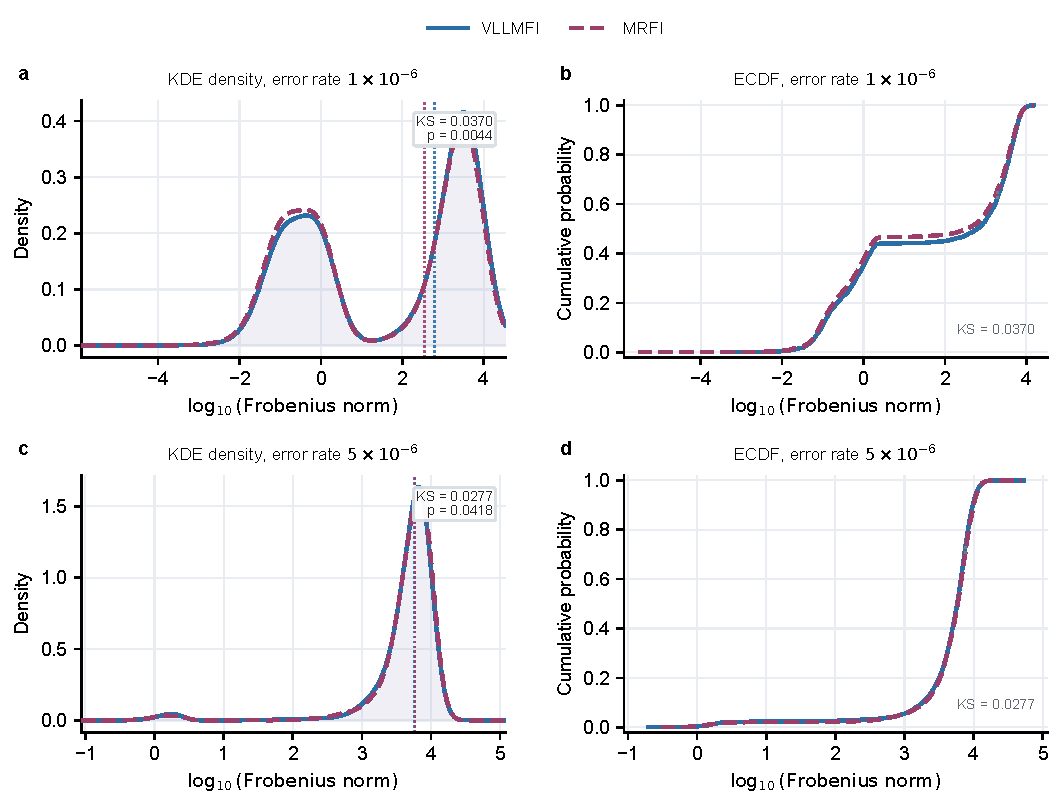
\includegraphics[width=\columnwidth]{fig_exp1_frob_distribution.pdf}
    \caption{\textbf{Tensor-level calibration against MRFI.}
    vLLM-FI produces activation perturbation distributions that closely match MRFI under different bit flip error rates.}
    \label{fig:exp1_frob_distribution}
\end{figure}

\textbf{Calibration Protocol.}
We calibrated vLLM-FI against MRFI at both the output and tensor levels. For each calibration setting, we performed five repetitions of 1,000 fault-injection trials on the same input sample. In both tools, all faults targeted the \texttt{down\_proj} module of the eighth model layer. For output-level analysis, we recorded whether the model produced the correct final output. For tensor-level analysis, we recorded the target-layer activations before and after fault injection.

\textbf{Output-Level Calibration.}
Figure~\ref{fig:exp1_consistency_analysis} compares the output-level fault effects produced by MRFI and vLLM-FI under different bit-flip error rates. The fault-injection (FI) correct rate is defined as the proportion of trials in which the model still produces the correct output after fault injection. Across all tested error rates, vLLM-FI closely matched MRFI, with a mean correlation coefficient of $r=0.999$ and a maximum absolute difference of only 0.62 percentage points. These results indicate that vLLM-FI reproduces the output-level fault effects of MRFI while operating on the native vLLM inference path.

\textbf{Tensor-Level Calibration.}
Agreement in final-output correctness does not necessarily imply that the two tools produce similar intermediate perturbations. We therefore compared the changes in the target-layer activation matrices before and after fault injection. Figure~\ref{fig:exp1_frob_distribution} presents the distributions of the Frobenius norms of the activation changes produced by MRFI and vLLM-FI. Panels (a) and (b) show the kernel density estimate (KDE) and empirical cumulative distribution function (ECDF) curves at a bit-flip error rate of $1\times10^{-6}$, whereas panels (c) and (d) show the corresponding results at $5\times10^{-6}$. At both error rates, the two tools produced highly overlapping distributions. The low Kolmogorov--Smirnov (KS) statistics further indicate close agreement between the distributions of their activation-change magnitudes.

Taken together, the output-level and tensor-level analyses show that, under the tested settings, vLLM-FI closely matches MRFI in both final-output correctness and the distribution of activation-change magnitudes. This agreement supports the use of vLLM-FI in the subsequent large-scale experiments.

\begin{figure}[t]
    \centering
    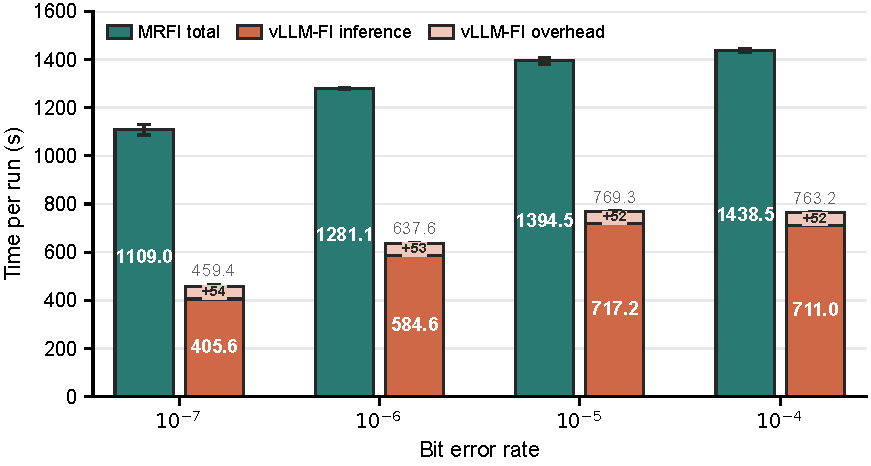
\includegraphics[width=\columnwidth]{exp1_mrfi_vllmfi_runtime_comparison.pdf}
\caption{\textbf{End-to-end runtime of MRFI and vLLM-FI.}
Bars show the mean runtime per run, with error bars denoting the standard deviation. The vLLM-FI runtime is divided into inference time and other runtime overhead.}
    \label{fig:mrfi_vllmfi_runtime}
\end{figure}

\textbf{End-to-End Runtime Comparison.}
We further compare the execution time of MRFI and vLLM-FI when faults are injected into all \texttt{down\_proj} modules in the model. The evaluated bit-flip error rates range from $10^{-7}$ to $10^{-4}$. Figure~\ref{fig:mrfi_vllmfi_runtime} reports the mean wall-clock time per run, with error bars indicating the sample standard deviation.

Across all tested error rates, vLLM-FI requires between $7.66$ and $12.82$ minutes per run, compared with $18.48$ to $23.98$ minutes for MRFI. This corresponds to a wall-clock time reduction of $44.8\%$--$58.6\%$, or a speedup of $1.81\times$--$2.41\times$. Model inference accounts for $88.3\%$--$93.2\%$ of the total vLLM-FI runtime, while the remaining runtime overhead remains nearly constant at approximately $52.1$--$53.8$ seconds. These results demonstrate that vLLM-FI reduces the end-to-end cost of repeated fault-injection experiments under the evaluated all-\texttt{down\_proj} injection workload.


\begin{figure}[t]
    \centering
    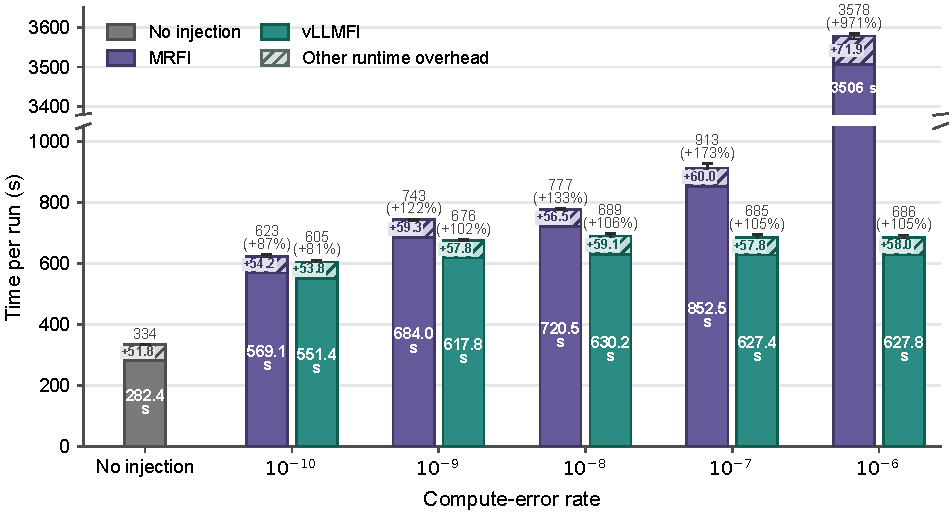
\includegraphics[width=\columnwidth]{extended_compute_error_runtime_comparison.pdf}
    \caption{\textbf{Controlled runtime comparison of MRFI-style and CUDA-based injection backends.}
    Mean runtime is reported for LLaMA-3.1-8B on GSM8K under compute-fault injection across all \texttt{down\_proj} modules. Percentages show increases over the no-injection baseline; the broken y-axis displays the MRFI-style result at $10^{-6}$.}
    \label{fig:controlled_injection_runtime}
\end{figure}

\textbf{Controlled Comparison of Injection Backends.}
To isolate the efficiency of the injection implementation from differences between inference frameworks, we ported the fault-injection logic of MRFI into the vLLM-FI runtime. We evaluate LLaMA-3.1-8B on GSM8K and inject compute faults into the outputs of all \texttt{down\_proj} modules. A fault-free execution is included as the baseline, and the evaluated compute-error rates range from $10^{-10}$ to $10^{-6}$.

Figure~\ref{fig:controlled_injection_runtime} shows that the runtime advantage of the CUDA backend increases with the error rate. At $10^{-10}$, the MRFI-style and CUDA backends require $623.3$ and $605.2$ seconds per run, respectively, corresponding to a modest reduction of $2.9\%$. As the error rate increases from $10^{-9}$ to $10^{-6}$, the runtime of the MRFI-style backend increases from $743.3$ to $3577.9$ seconds. In contrast, the CUDA backend remains between $675.6$ and $689.3$ seconds. At $10^{-6}$, the CUDA backend reduces wall-clock time by $80.8\%$ and achieves a $5.22\times$ speedup over the MRFI-style backend.

Taken together, the two runtime comparisons show that vLLM-FI reduces the end-to-end cost of repeated fault-injection experiments relative to MRFI and scales more efficiently as the fault rate increases. Under the evaluated workload targeting all \texttt{down\_proj} layers, the CUDA backend maintains comparatively stable runtime across the tested error rates, whereas the MRFI-style backend becomes substantially more expensive, yielding a maximum speedup of $5.22\times$ at $10^{-6}$. These results support the use of vLLM-FI for large-scale fault-injection campaigns.

\subsection{Reliability Assessment across Downstream Tasks}

\begin{figure}[t]
    \centering
    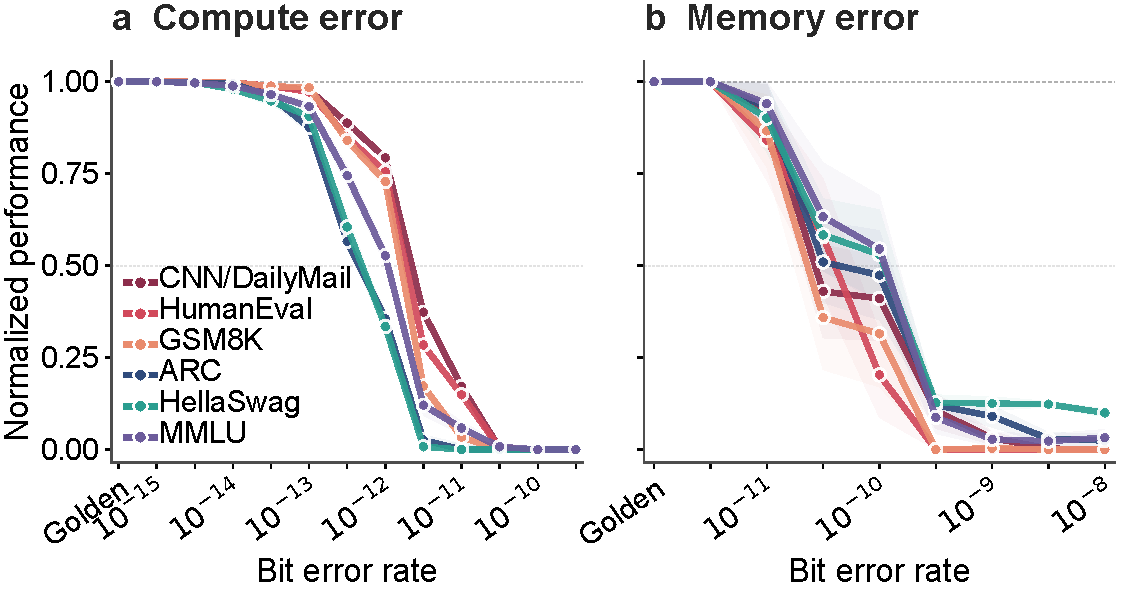
\includegraphics[width=\columnwidth]{fig_error_degradation_compute_memory.pdf}
    \caption{\textbf{Global degradation trends under compute and memory faults.}
    Compute and memory faults exhibit distinct reliability cliffs across downstream tasks.}
    \label{fig:error_degradation_compute_memory}
\end{figure}


\textbf{Global Degradation Trends.}
We characterize the reliability of Llama under compute and memory faults in two steps. The injection scope covers all layers of the Llama model, and multiple fault-injection runs are performed at each BER. We first scan a wide BER range over the full model to observe the global performance trajectory as the error rate increases. We then focus on the critical interval where the model transitions from near-baseline behavior to clear degradation and perform task-level evaluations within this interval.

Figure~\ref{fig:error_degradation_compute_memory} presents normalized task performance under compute and memory faults across downstream benchmarks. Both fault types exhibit localized reliability cliffs. The following task level analysis uses fault specific BER intervals selected from these global degradation trends.

\begin{figure}[t]
    \centering
    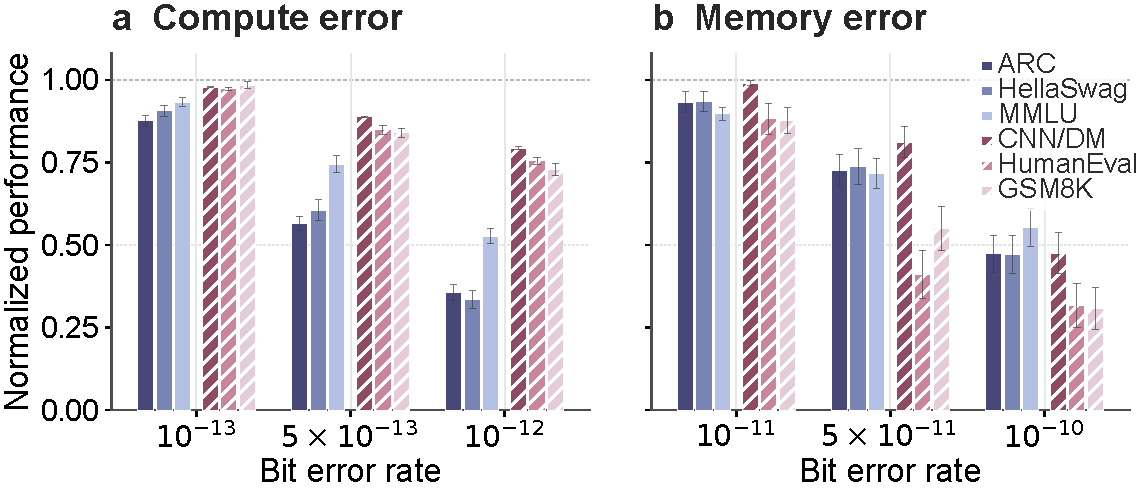
\includegraphics[width=\columnwidth]{fig_shadow_interval_task_performance.pdf}
    \caption{\textbf{Task level performance within critical BER intervals.}
    Compute and memory faults show opposite vulnerability patterns across multiple choice and generative tasks.}
    \label{fig:shadow_interval_task_performance}
\end{figure}


\textbf{Task Vulnerability Across Fault Models.} Figure~\ref{fig:shadow_interval_task_performance} presents task level performance within the critical BER intervals identified from the global degradation trends. Panel (a) shows normalized performance under compute faults from $10^{-13}$ to $10^{-12}$, while Panel (b) shows normalized performance under memory faults from $10^{-11}$ to $10^{-10}$. The evaluated benchmarks include three multiple choice tasks, ARC, HellaSwag, and MMLU, and three generative tasks, CNN/DailyMail, HumanEval, and GSM8K.

Restricting the analysis to the selected critical BER intervals reveals a fault-dependent reversal in task vulnerability, as summarized below.

\begin{observationbox}{Observation 1: Task vulnerability reverses across fault models}
Within the selected BER intervals, generative tasks are more vulnerable to memory faults, whereas multiple-choice tasks are more vulnerable to compute faults.
\end{observationbox}



This reversal can be explained by the different persistence and propagation behavior of the two fault models. Memory faults directly corrupt model weights, and their effects persist across subsequent layer computations. For generative tasks, such persistent perturbations can further affect intermediate states during auto regressive decoding, allowing errors to accumulate over multiple generation steps. In contrast, multiple choice tasks usually evaluate a fixed set of candidate answers and map model outputs to a discrete option space. Their final predictions are affected only when the perturbation changes candidate ranking or crosses a decision boundary.

Compute faults exhibit a different behavior because they are closer to local transient perturbations. A single activation perturbation usually affects a specific token or local output position, rather than persisting across subsequent inference steps as weight corruption does. For generative tasks, this local perturbation may be partially diluted by later contextual information, resulting in smoother performance degradation. For multiple choice tasks, however, the final answer often depends on key token representations and candidate logits. Local activation anomalies can therefore more directly change rankings near the decision boundary.


\begin{figure}[t]
    \centering
    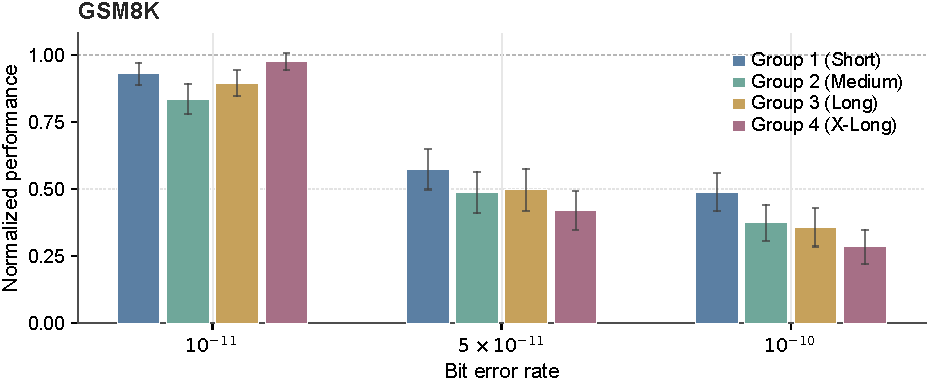
\includegraphics[width=\columnwidth]{fig_gsm8k_length_memory_error.pdf}
    \caption{\textbf{Effect of output length on GSM8K reliability under memory faults.}
    Longer generations show stronger degradation under persistent weight perturbations.}
    \label{fig:gsm8k_length_memory_error}
\end{figure}

\textbf{Effect of Generation Length.}
To further investigate why generative tasks are more sensitive to memory faults, we perform a sequence length ablation on GSM8K. GSM8K samples are first filtered to include only baseline correct examples. They are then grouped according to the token length of the model generated answer, measured by the Llama 3.1 8B tokenizer. Based on this length, the samples are divided into four groups: Short, Medium, Long, and X Long. Each group is evaluated under the same memory fault setting within the critical BER interval from $10^{-11}$ to $10^{-10}$.

As shown in Figure~\ref{fig:gsm8k_length_memory_error}, short output groups maintain higher normalized performance across the tested BER range, whereas longer output groups degrade more rapidly. This trend supports the interpretation that persistent weight perturbations can accumulate through repeated auto regressive decoding. Short sequence tasks may complete generation before the accumulated error becomes severe, whereas long sequence tasks undergo more decoding steps and are therefore more exposed to the persistent effects of memory faults.

\begin{observationbox}{Observation 2: Longer generation increases vulnerability to memory faults}
Under memory faults, GSM8K samples with longer target outputs exhibit more pronounced performance degradation. This indicates that the vulnerability of generative tasks is positively associated with the number of auto regressive decoding steps.
\end{observationbox}


\subsection{Reliability Assessment of Quantization Methods}

This section focuses on weight quantization, which is widely used in LLM deployment because it reduces memory footprint and bandwidth pressure.

\begin{figure}[t]
    \centering
    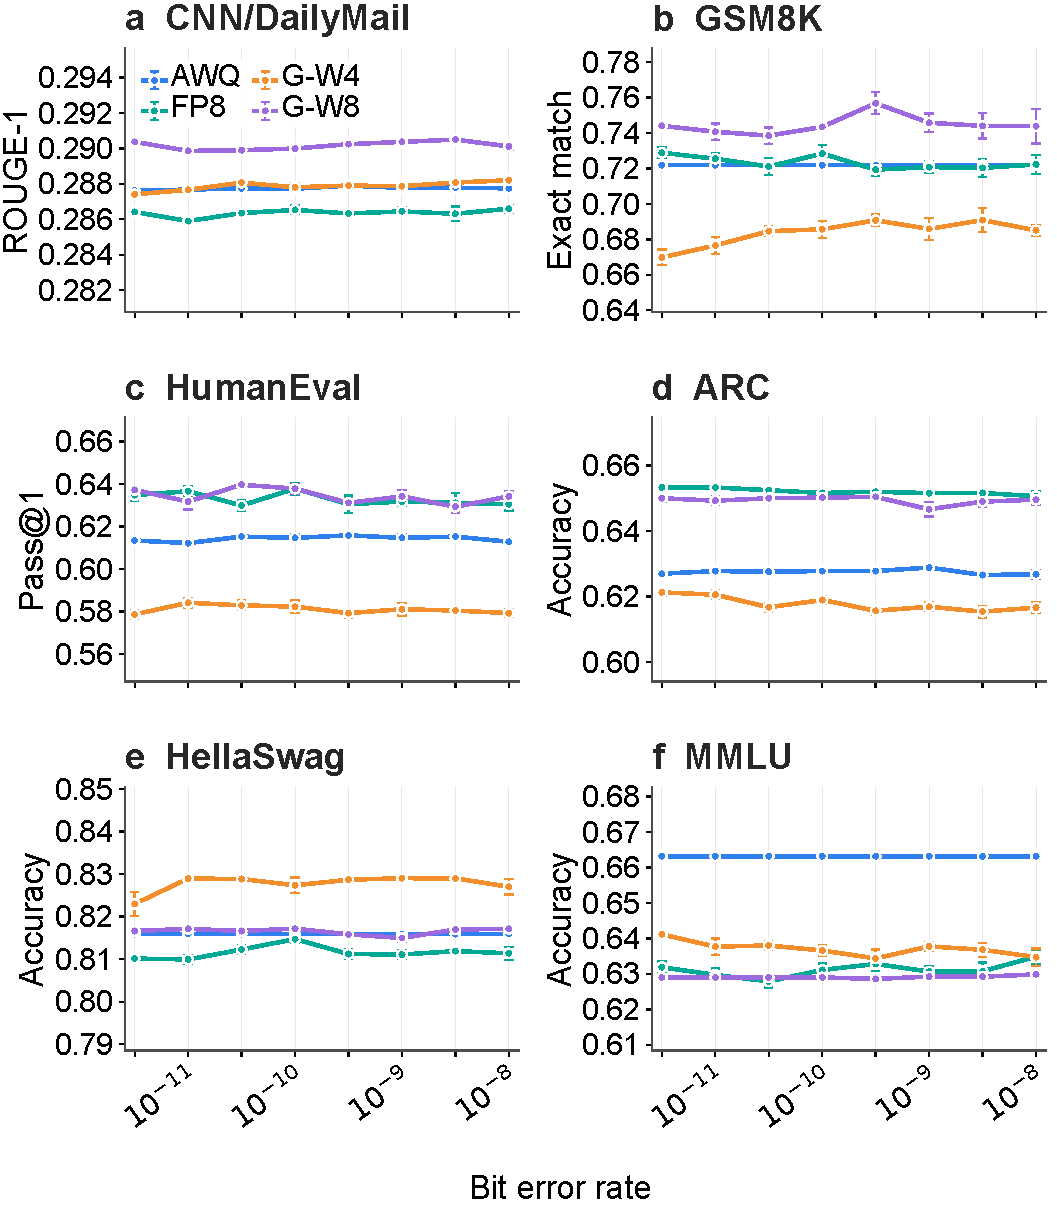
\includegraphics[width=\columnwidth]{fig_quantization_memory_error.pdf}
    \caption{\textbf{Reliability of weight quantized models under memory faults.}
    Quantized weight representations show relatively stable performance across downstream tasks.}
    \label{fig:quantization_memory_error}
\end{figure}

Figure~\ref{fig:quantization_memory_error} compares FP8, AWQ, GPTQ W4, and GPTQ W8 under memory faults across six downstream tasks. As in the preceding experiments, the fault-injection scope covers all model layers for each quantization configuration. The evaluated BER range spans from $5\times10^{-12}$ to $10^{-8}$. Across this range, weight-only quantized models show relatively stable performance, with no sharp degradation trend across the tested tasks.

\begin{observation}
\textbf{Observation 3:} Within the BER range evaluated in this study, weight  quantized models show relatively stable performance under memory faults, with no sharp degradation trend across the tested downstream tasks.
\end{observation}


This behavior may partly arise from the bounded representations used by quantized weights. Although INT4, INT8, and FP8 use different numerical encodings, their stored values are mapped to computation values through scaling or format conversion. For finite corrupted values, these representation ranges can limit the magnitude of resulting perturbations compared with FP16 or BF16, whose exponent-bit flips may produce much larger outliers or non-finite values.


Therefore, under memory faults, weight quantization may reduce the amplification of weight corruption by acting as an implicit numerical range constraint.


\subsection{Reliability Assessment under Different Communication Strategies}

This section investigates how communication-related faults affect model reliability during distributed inference. Unlike local computation faults, communication faults can propagate through cross-rank aggregation or inter-stage activation transfers. Consequently, their end-to-end effects may vary with the bit error rate (BER), communication frequency, synchronization scope, and fault propagation path of each parallelization strategy. To characterize these strategy-level differences, we compare tensor parallelism and pipeline parallelism under their native communication workloads.


\begin{figure}[t]
    \centering
    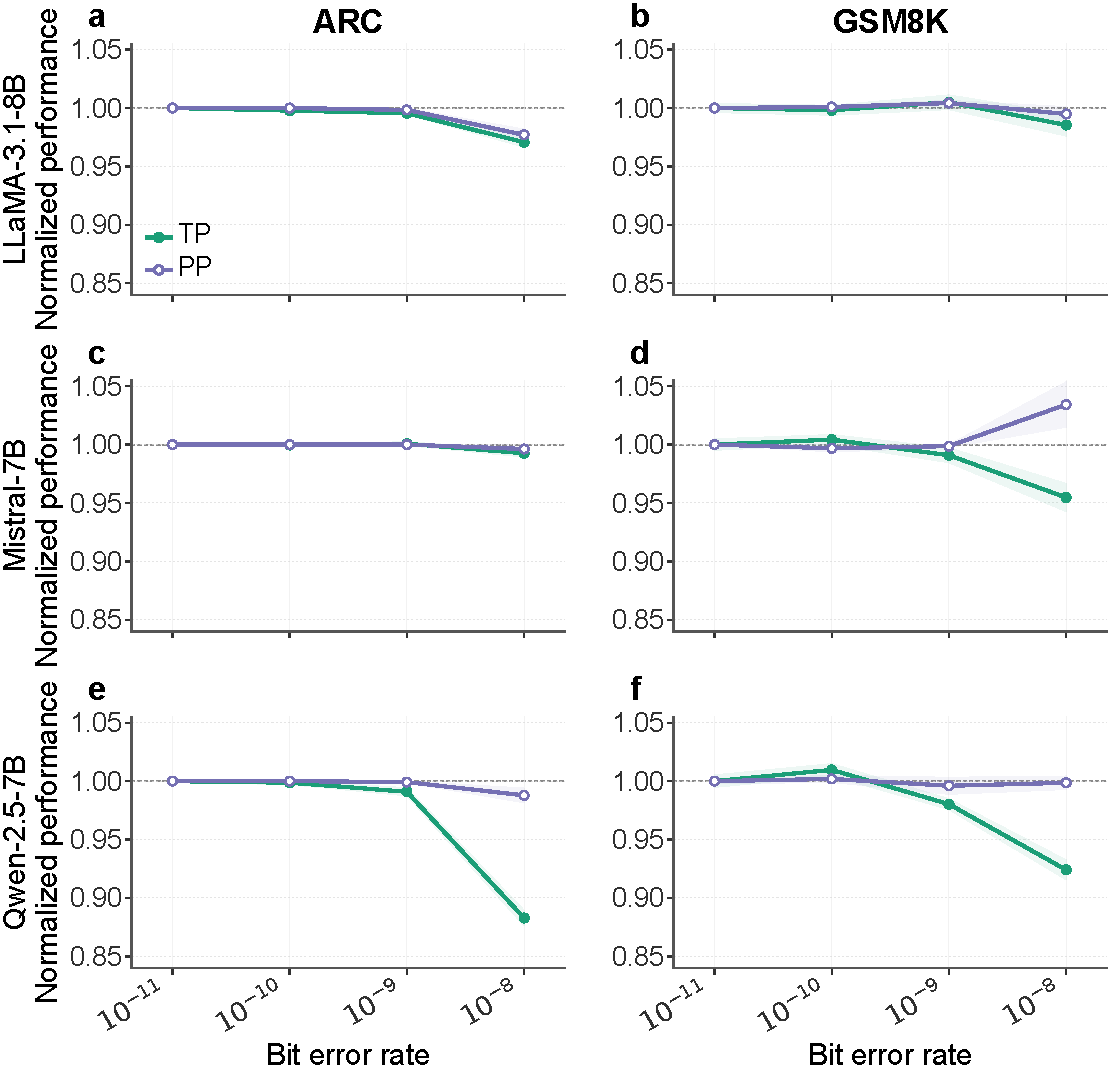
\includegraphics[width=\columnwidth]{fig_exp5_tp_pp_reliability_3x2_linechart.pdf}
    \caption{\textbf{End-to-end reliability of tensor parallelism and pipeline parallelism under communication-related faults.}
    Normalized performance is reported for LLaMA-3.1-8B, Mistral-7B, and Qwen-2.5-7B on ARC and GSM8K at BER points evaluated for both strategies. Solid blue lines denote tensor parallelism, whereas dashed orange lines denote pipeline parallelism.}
    \label{fig:tp_pp_communication}
\end{figure}

Figure~\ref{fig:tp_pp_communication} compares the performance degradation of tensor parallelism and pipeline parallelism under communication-related faults. To ensure a consistent horizontal comparison, we report only the BER values evaluated for both strategies. At the highest shared BER of $10^{-8}$, tensor parallelism and pipeline parallelism achieved mean normalized performances of $0.952$ and $0.998$, respectively. This result corresponds to an average advantage of $4.64$ percentage points for pipeline parallelism. Across individual tasks, pipeline parallelism exceeded tensor parallelism by $3.83$ percentage points on ARC and $5.45$ percentage points on GSM8K. The largest gap occurred for Qwen-2.5-7B on ARC, where tensor parallelism and pipeline parallelism achieved normalized performances of $0.883$ and $0.988$, respectively, corresponding to a difference of $10.50$ percentage points.

\begin{observation}
\textbf{Observation 4:} Within the evaluated BER range and native communication workloads, pipeline parallelism exhibits higher end-to-end reliability than tensor parallelism.
\end{observation}

The observed reliability gap may arise from the distinct communication patterns of the two strategies. Tensor parallelism invokes collective operations within multiple Transformer layers. At the same per-bit error rate, its higher communication frequency exposes more transmitted values to corruption, while cross-rank aggregation may spread corrupted values across multiple ranks. By contrast, pipeline parallelism mainly transfers activations between adjacent stages, so communication is concentrated at stage boundaries and faults primarily affect downstream stages.

These results characterize the end-to-end reliability of each parallelization strategy under its native communication workload. The normalized performance slightly above \(1.0\) for Mistral-7B on GSM8K under pipeline parallelism reflects run-to-run variation relative to the fault-free baseline and does not indicate a fault-induced performance gain.


% This section investigates how communication-related faults affect model reliability during distributed inference. Unlike faults in local computation, communication faults can propagate through cross-rank aggregation or inter-stage activation transfers. Their effects therefore depend not only on the bit error rate, but also on the communication frequency, synchronization scope, and fault propagation path associated with each parallelization strategy. We conduct two comparative experiments. First, we examine whether tensor parallelism introduces additional reliability risks relative to a baseline configuration without tensor parallelism. Second, we compare the degradation behavior of tensor parallelism and pipeline parallelism under communication-related faults.


% \begin{figure}[t]
%     \centering
%     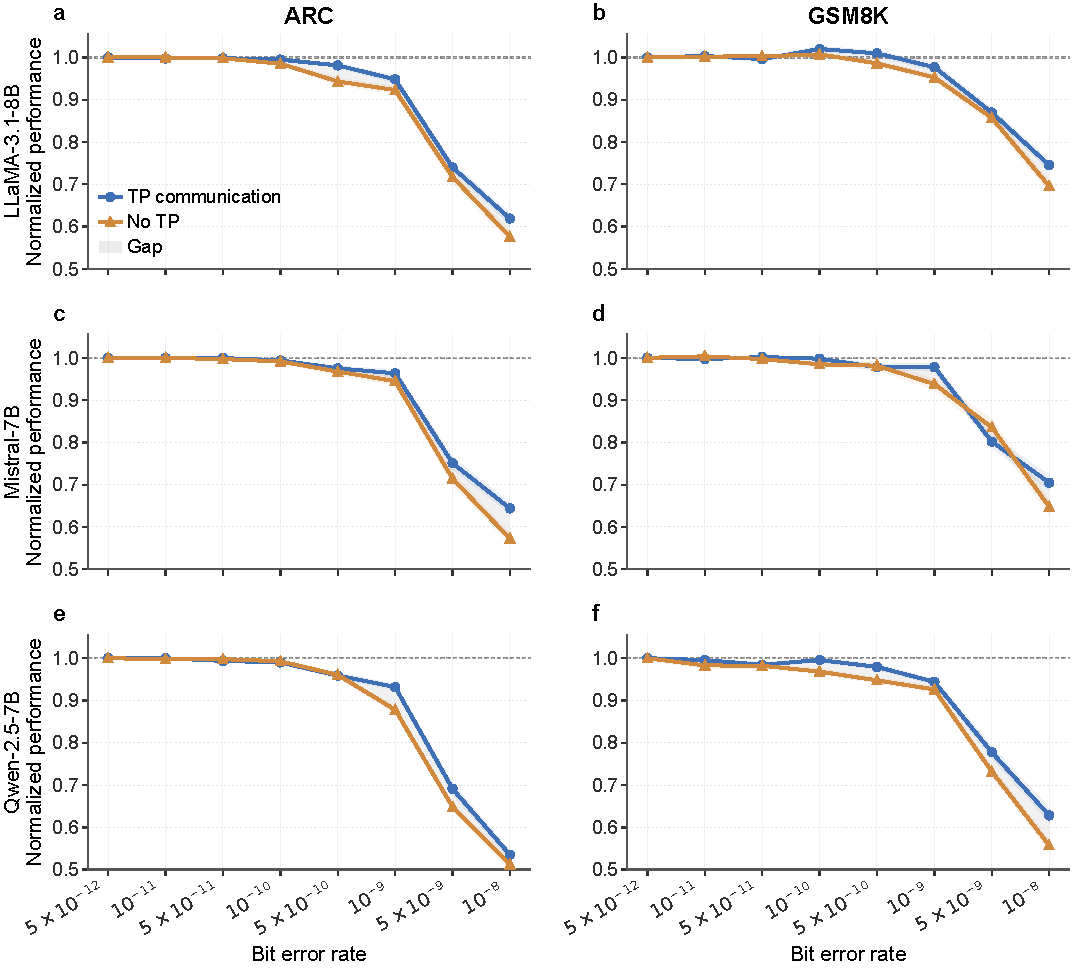
\includegraphics[width=\columnwidth]{fig_exp5_tp_no_tp_downproj_gap.pdf}
%     \caption{\textbf{Effect of tensor-parallel communication on fault sensitivity.}
%     Normalized performance of LLaMA-3.1-8B, Mistral-7B, and Qwen-2.5-7B on ARC and GSM8K under fault injection at the \texttt{down\_proj} layer. Blue curves denote the tensor-parallel communication setting, orange curves denote the setting without tensor parallelism, and shaded regions indicate the performance gap.}
%     \label{fig:tp_no_tp_communication}
% \end{figure}

% Figure~\ref{fig:tp_no_tp_communication} compares the reliability of tensor parallelism with that of the baseline configuration without tensor parallelism when faults are injected at the \texttt{down\_proj} layer. At low bit error rates, both configurations maintain normalized task performance close to $1.0$. As the bit error rate increases, both configurations exhibit noticeable degradation. Nevertheless, tensor parallelism preserves higher normalized performance across most model--task combinations.

% At the highest tested bit error rate of $10^{-8}$, tensor parallelism achieves an average normalized performance of $0.599$ on ARC, compared with $0.553$ for the baseline configuration. On GSM8K, the corresponding values are $0.693$ and $0.634$, respectively. The largest difference is observed for Mistral-7B on ARC, where tensor parallelism retains a normalized performance of $0.644$, whereas the baseline configuration achieves $0.572$, corresponding to a difference of $7.14$ percentage points.

% \begin{observation}
% \textbf{Observation 4:} Under the evaluated \texttt{down\_proj} injection setting and bit error rate range, tensor parallelism exhibits stronger fault tolerance than the baseline configuration without tensor parallelism.
% \end{observation}

% This behavior may be associated with the partial-result aggregation used by the tensor-parallel implementation of \texttt{down\_proj}. In the row-parallel configuration considered in this study, each rank computes a partial projection result, after which the partial results are aggregated through collective communication. A fault injected before this aggregation initially perturbs only the local contribution produced by one rank, which is subsequently combined with the contributions from the remaining ranks. By contrast, in the baseline configuration without tensor parallelism, the injected fault directly perturbs the complete projection result.

% Because partial and complete tensors can differ in their numerical distributions and dynamic ranges, an identical bit flip does not necessarily induce a perturbation of the same numerical magnitude in the two configurations. This difference provides a plausible explanation for the higher reliability observed with tensor parallelism. However, the effect may depend on the injection location, tensor-parallel degree, numerical format, and communication implementation, and should therefore not be generalized to all tensor-parallel configurations.



% \begin{figure}[t]
%     \centering
%     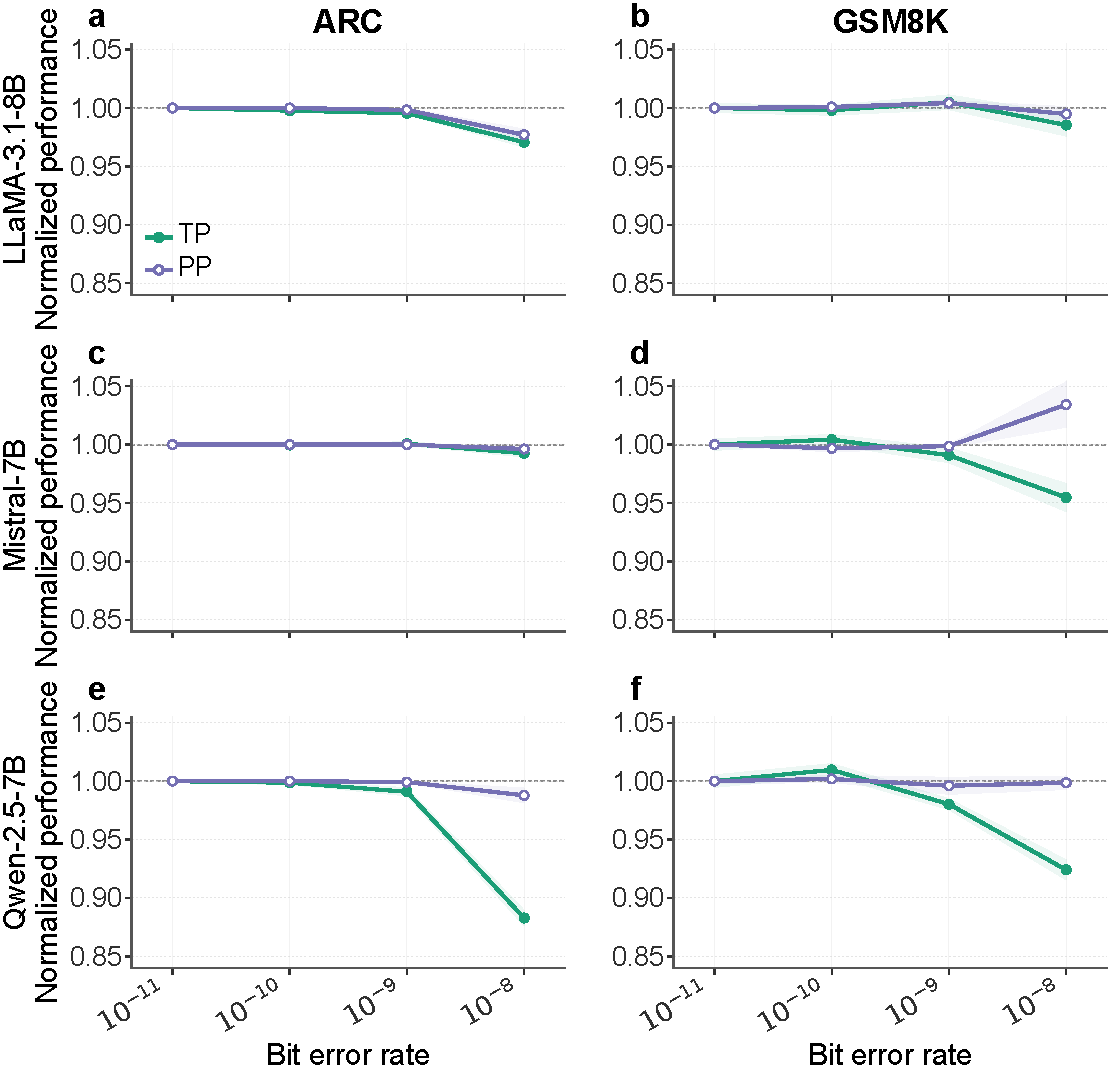
\includegraphics[width=\columnwidth]{fig_exp5_tp_pp_reliability_3x2_linechart.pdf}
%     \caption{\textbf{Reliability comparison between tensor parallelism and pipeline parallelism under communication related faults.}
%     Normalized performance is reported for LLaMA-3.1-8B, Mistral-7B, and Qwen-2.5-7B on ARC and GSM8K using shared BER points. Solid blue lines denote tensor parallelism, and dashed orange lines denote pipeline parallelism.}
%     \label{fig:tp_pp_communication}
% \end{figure}

% Figure~\ref{fig:tp_pp_communication} further compares tensor parallelism and pipeline parallelism under communication-related faults. To ensure a consistent horizontal comparison, the figure includes only the bit error rates evaluated for both strategies. At the highest tested bit error rate of $10^{-8}$, tensor parallelism and pipeline parallelism achieve average normalized performances of $0.952$ and $0.998$, respectively, giving pipeline parallelism an average advantage of $4.64$ percentage points. When evaluated separately, pipeline parallelism exceeds tensor parallelism by $3.83$ percentage points on ARC and $5.45$ percentage points on GSM8K. The largest difference occurs for Qwen-2.5-7B on ARC, where tensor parallelism and pipeline parallelism achieve normalized performances of $0.883$ and $0.988$, respectively, corresponding to a difference of $10.50$ percentage points.

% \begin{observation}
% \textbf{Observation 5:} Under the evaluated communication fault conditions, pipeline parallelism exhibits stronger fault tolerance than tensor parallelism.
% \end{observation}

% The observed difference may arise from the distinct communication exposure of the two strategies. Tensor parallelism typically invokes collective communication within multiple Transformer layers, resulting in frequent synchronization and a broad cross-rank fault propagation scope. Pipeline parallelism, in contrast, primarily transfers intermediate activations between adjacent pipeline stages. Its communication is therefore concentrated at stage boundaries and involves fewer communication sites.

% Consequently, under the same per-bit error rate, tensor parallelism may experience a larger number of corrupted communicated values because of its greater communication volume and frequency. Communication faults may also affect multiple ranks through collective aggregation, whereas faults in pipeline parallelism propagate mainly through the downstream stages following the affected boundary.

% Accordingly, this experiment evaluates the end-to-end reliability of each strategy under its native communication workload, rather than its intrinsic sensitivity to an identical number of injected faults. A more strictly controlled comparison would additionally normalize the total number of injected faults or the total volume of communicated data. Normalized values slightly above $1.0$, such as those observed for pipeline parallelism on Mistral-7B and GSM8K, reflect run-to-run variability around the normalization reference and should not be interpreted as fault-induced performance improvements.



\subsection{Reliability Analysis under Model Parallelism}

This section analyzes whether different device positions within TP and PP exhibit different reliability under memory faults and compute faults, focusing on rank level vulnerability in TP and stage level vulnerability in PP.

\begin{figure}[t]
    \centering
    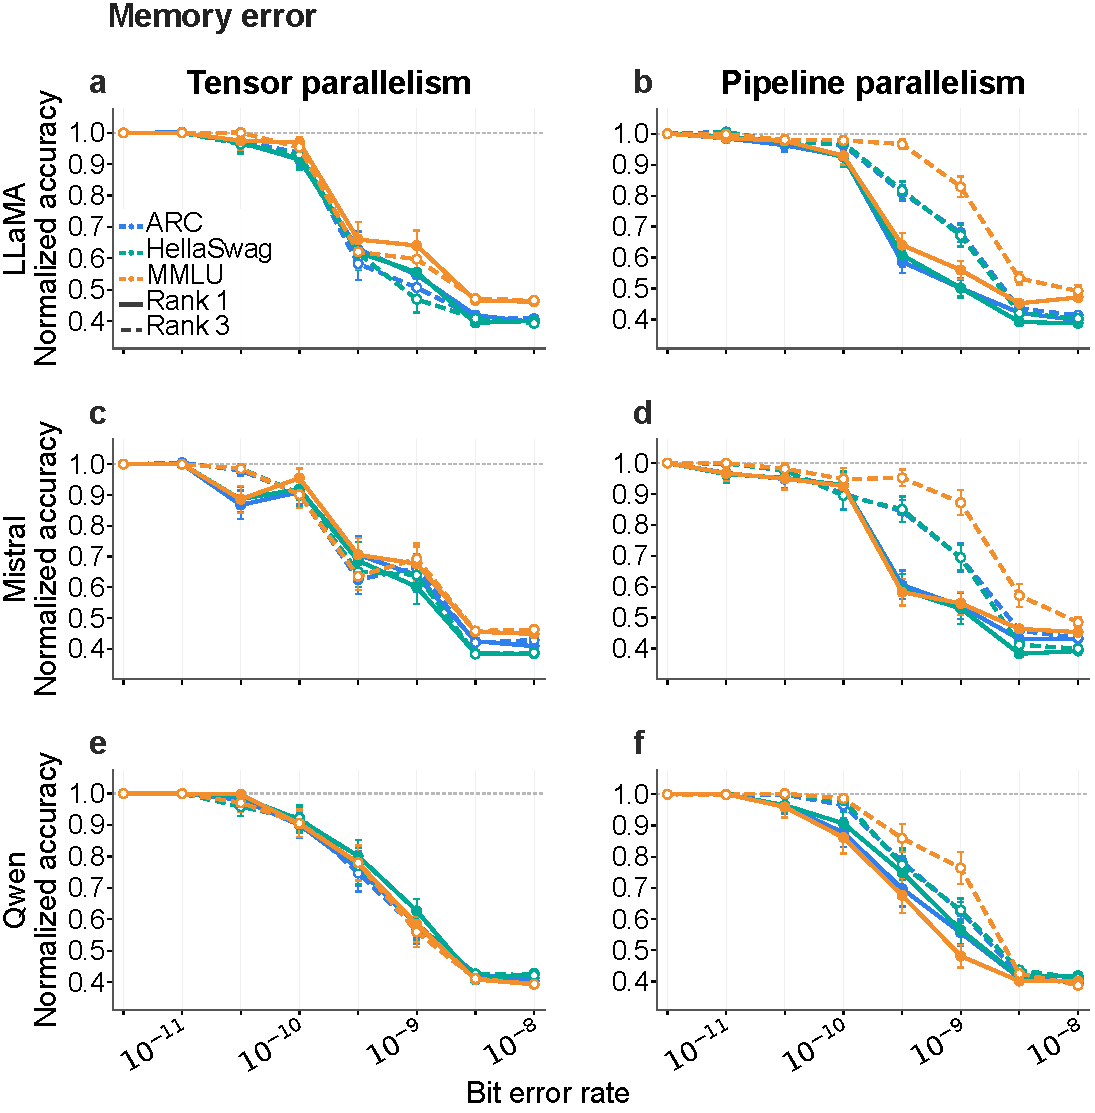
\includegraphics[width=\columnwidth]{fig_exp4_memory_compute_split_memory_error.pdf}
    \caption{\textbf{Rank and stage sensitivity under memory faults.}
    PP exhibits stronger position dependent vulnerability than TP.}
    \label{fig:parallel_memory_error}
\end{figure}

\begin{figure}[t]
    \centering
    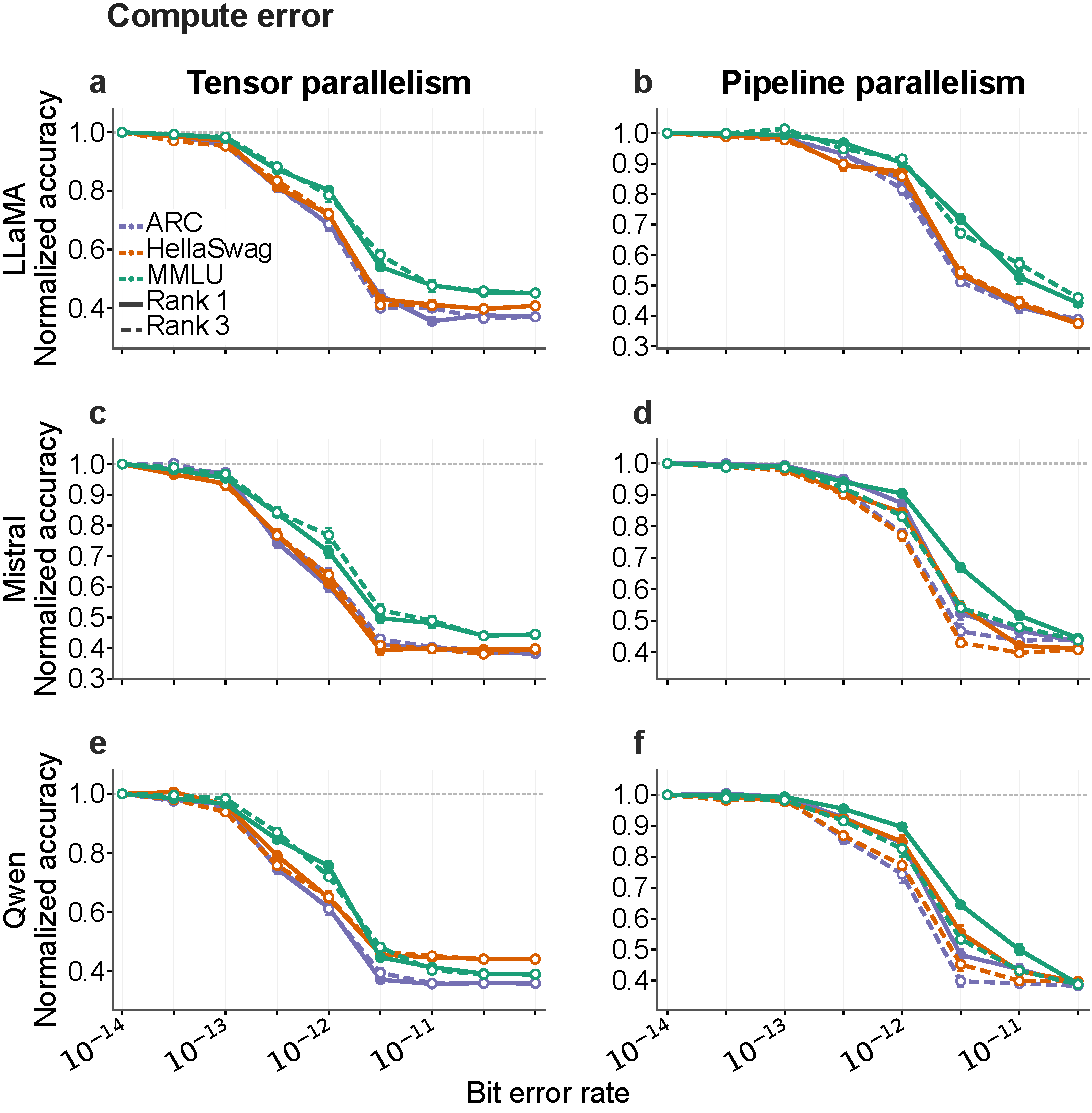
\includegraphics[width=\columnwidth]{fig_exp4_memory_compute_split_compute_error.pdf}
    \caption{\textbf{Rank and stage sensitivity under compute faults.}
    Later PP stages are more sensitive, while TP ranks show similar trends.}
    \label{fig:parallel_compute_error}
\end{figure}

As shown in Figures~\ref{fig:parallel_memory_error} and~\ref{fig:parallel_compute_error}, we evaluate LLaMA, Mistral, and Qwen under TP and PP configurations on ARC, HellaSwag, and MMLU. The parallel degree is fixed to 4. Fault-injection experiments are conducted separately on each of the four ranks. For each target rank, the injection scope covers all model layers or layer partitions assigned to that rank. Figures~10 and~11 report the results for Rank~1 and Rank~3, with the TP results shown in the left column and the PP results in the right column. This setup allows us to assess the effect of device position on model reliability.

\begin{observation}
\textbf{Observation 6:} Under TP, Rank 1 and Rank 3 show relatively similar degradation trends under both memory faults and compute faults. Under PP, reliability becomes more stage dependent: earlier stages are more sensitive to memory faults, whereas later stages show stronger sensitivity to compute faults.
\end{observation}

This difference is consistent with the partitioning structure of the two parallel strategies. TP partitions computation along tensor dimensions, so different ranks participate in the same layer computation with relatively symmetric roles. As a result, injecting faults into different TP ranks tends to produce similar degradation trends. In contrast, PP partitions the model along network depth, so different stages occupy different positions in the forward propagation path.

For memory faults, an error in an earlier PP stage corrupts the hidden state of a token earlier in the forward path. The perturbed representation is then propagated through more subsequent layers, increasing its chance to affect downstream representations and final predictions. In contrast, a memory fault in a later stage has a shorter propagation path before the output, which limits its opportunity to influence the model computation. For compute faults, the effect of an early local activation perturbation may be partially attenuated by later normalization, residual transformations, and layer wise computation. Faults injected into later PP stages are closer to the output and therefore have fewer subsequent layers in which their effects can be diluted, making them more directly visible in the final prediction.

\section{Conclusion}
\label{sec:conclusion}

This paper presented vLLM-FI, a fault-injection and reliability-evaluation framework integrated with the native vLLM runtime. The framework extends fault modeling to account for computational workload and inter-device communication, coordinates injection across distributed Workers, and performs in-place bit flips on GPU-resident tensors. Together with support for quantized inference and integration with \texttt{lm-evaluation-harness}, these capabilities enable systematic reliability evaluation across downstream tasks and parallel execution configurations.

Experiments demonstrate both the consistency and efficiency of vLLM-FI under the evaluated settings. Its fault-injection correct rates differ from MRFI by at most 0.62 percentage points, while its end-to-end runtime achieves a $1.81\times$--$2.41\times$ speedup. With the inference runtime held fixed, the CUDA backend achieves up to a $5.22\times$ speedup in total experiment runtime over an MRFI-style CPU-mediated backend under compute-fault injection. The reliability study further shows that task vulnerability depends on the fault model, longer generation increases sensitivity to persistent weight corruption, and parallel execution introduces distinct communication and stage-dependent fault effects. These findings motivate evaluation across multiple tasks and deployment configurations rather than reliance on a single benchmark. By reducing experimental cost and connecting distributed fault injection with standardized task evaluation, vLLM-FI provides a practical foundation for studying LLM reliability and informing selective protection and deployment decisions.

\begingroup
    % 1. 字体调整：期刊通常使用 \footnotesize 或 \small
    \footnotesize
    
    % 2. 行距调整：让列表更紧凑，符合期刊双栏排版习惯
    \setlength{\itemsep}{1pt} 
    \setlength{\parskip}{0pt} 
    
    % 3. 样式设置
    \bibliographystyle{IEEEtran}
    
    % 4. 加载缩写库 + 你的文件
    % 注意：IEEEabrv 必须放在你的文件名之前
    \bibliography{IEEEabrv, sample} 
\endgroup


\end{document}



